% Standalone Overleaf entry point for the anonymous CHI review format.
% Upload this file with references.bib and the figure/ directory, then set
% sigconf-authordraft.tex as the project's Main document.
\documentclass[manuscript,review,anonymous]{acmart}

\citestyle{acmnumeric}
\setcopyright{none}
\settopmatter{printacmref=true}
\renewcommand\footnotetextcopyrightpermission[1]{}
\setlength{\headheight}{21pt}
\copyrightyear{2027}
\acmYear{2027}

\usepackage{booktabs}       \usepackage{tabularx}       \usepackage{amsmath}        \usepackage{amsfonts}       \usepackage{nicefrac}       \usepackage{microtype}      \usepackage{enumitem}       \usepackage{tikz}           \usepackage{placeins}
\usetikzlibrary{positioning,arrows.meta,shapes.geometric,calc,decorations.pathreplacing,fit,backgrounds}



\title{Learning Human-Grounded Interaction Strategies for Interactive Agents
through Action-Mediated Language Policies}

\author{Yu Song}
\affiliation{%
  \institution{Shanghai Institute of AI for Education, East China Normal University}
  \city{Shanghai}
  \country{China}}

\author{Yutao Xie}
\affiliation{%
  \institution{Shanghai Institute of AI for Education, East China Normal University}
  \city{Shanghai}
  \country{China}}

\author{Jiaming Lan}
\affiliation{%
  \institution{Shanghai Institute of AI for Education, East China Normal University}
  \city{Shanghai}
  \country{China}}

\author{Ying Qian}
\affiliation{%
  \institution{Shanghai Institute of AI for Education, East China Normal University}
  \city{Shanghai}
  \country{China}}

\author{Yanjun Huang}
\affiliation{%
  \institution{Shanghai Institute of AI for Education, East China Normal University}
  \city{Shanghai}
  \country{China}}

\acmConference[CHI '27]{CHI Conference on Human Factors in Computing Systems}
  {2027}{Pittsburgh, PA, USA}


\begin{document}
\begin{abstract}
Interactive agents can generate fluent responses, yet the interaction strategy
behind each response typically remains implicit in end-to-end language
generation. This makes strategic choices---such as probing, guiding,
challenging, or building on prior contributions---difficult to learn from human
interaction, inspect, and coordinate across turns. We introduce Language-Action
Inverse Q-Learning (LA-IQL), an action-mediated framework that learns offline
from authentic classroom trajectories without online exploration or a
hand-designed scalar reward. LA-IQL separates rationale generation, selection
over human-readable interaction acts, and language realization. On held-out
K--12 lessons, the evaluated TD-regularized checkpoint exhibits less recurrent
behavior than its no-TD counterpart while maintaining similar local
human-pattern alignment. A metric-matched Markov control shows that strong local alignment
can arise without dialogue context, while semantic interventions indicate
context-sensitive policy behavior. Direct selection better matches held-out
human action patterns, whereas proposal-constrained re-ranking reduces
recurrence, revealing an alignment--repetition trade-off. Action mediation
thus makes long-horizon interaction strategies
explicitly inspectable beyond surface fluency.
\end{abstract}

\begin{CCSXML}
<ccs2012>
 <concept>
  <concept_id>10003120.10003121</concept_id>
  <concept_desc>Human-centered computing~Human computer interaction (HCI)</concept_desc>
  <concept_significance>500</concept_significance>
 </concept>
 <concept>
  <concept_id>10010147.10010257.10010293</concept_id>
  <concept_desc>Computing methodologies~Reinforcement learning</concept_desc>
  <concept_significance>300</concept_significance>
 </concept>
</ccs2012>
\end{CCSXML}

\ccsdesc[500]{Human-centered computing~Human computer interaction (HCI)}
\ccsdesc[300]{Computing methodologies~Reinforcement learning}

\keywords{human-grounded interaction, interactive agents,
action-mediated policy, offline imitation learning, dialogue strategy}

\begin{teaserfigure}
\centering
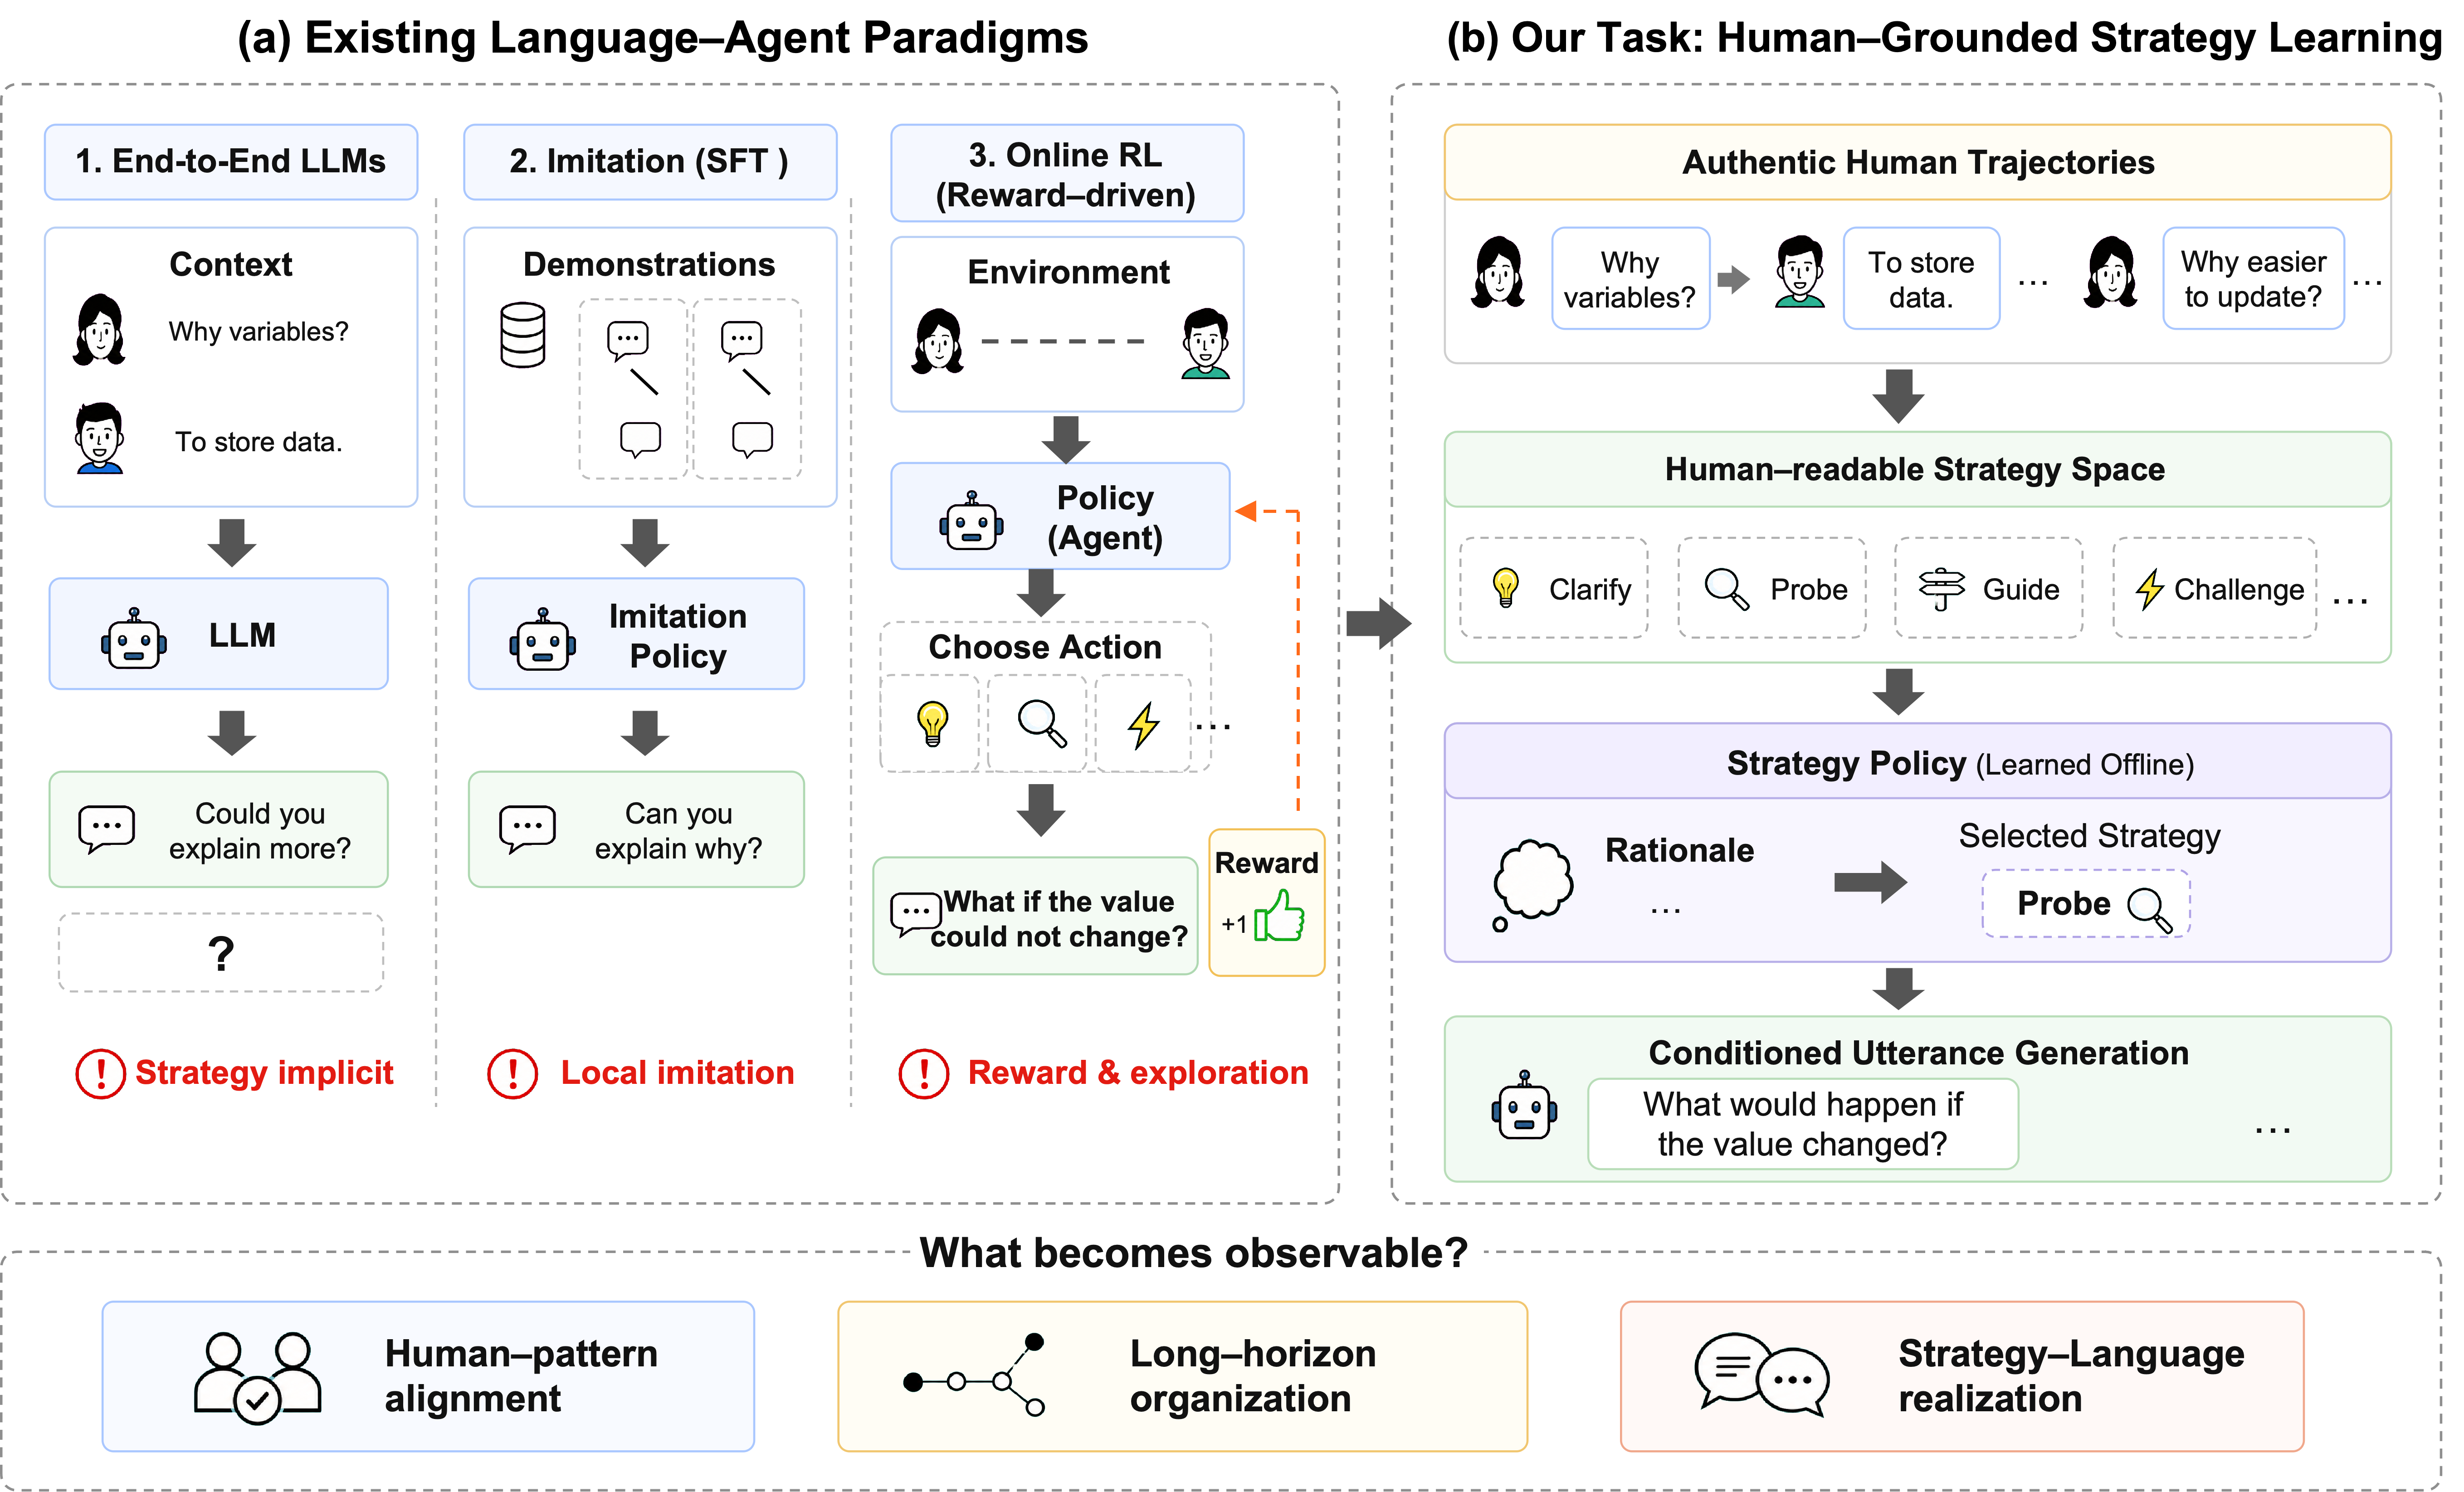
\includegraphics[width=\textwidth]{figure/teaser.png}
\caption{\textbf{Action mediation makes interaction strategy explicit and
inspectable.} End-to-end generation leaves strategy implicit, supervised
imitation emphasizes local reproduction, and online reinforcement learning
depends on reward design and exploration. LA-IQL instead learns offline from
authentic human trajectories over a human-readable strategy space, exposes a
rationale and selected strategy, and conditions utterance generation on that
choice. This explicit boundary makes human-pattern alignment, long-horizon
organization, and strategy--language realization separately observable.}
\Description{A comparison of four approaches to interactive-agent behavior. On
the left, end-to-end language models map context directly to an utterance,
supervised fine-tuning imitates demonstrations locally, and online
reinforcement learning selects actions using environmental rewards. On the
right, LA-IQL derives a human-readable strategy space from authentic human
trajectories, learns an offline strategy policy that produces a rationale and
selected action, and conditions utterance generation on that action. A bottom
row identifies three observable outcomes: human-pattern alignment,
long-horizon organization, and strategy--language realization.}
\label{fig:teaser}
\end{teaserfigure}
 
\maketitle

\section{Introduction}

Interactive agents have become woven into the fabric of everyday life. Voice
assistants field our questions, tutoring systems guide learners through
exercises, customer service bots resolve issues, and companion agents provide
social engagement. Across these diverse settings, dialogue serves as the
fundamental interface through which agents interpret human intent, negotiate
meaning, and accomplish tasks~\citep{park2023generative,xi2025rise}. The quality
of this dialogic interaction increasingly determines whether these systems feel
helpful, natural, and engaging, or mechanical, rigid, and unsatisfying.
These gaps between conversational capability and user expectations are
long-standing concerns in HCI~\citep{luger2016badpa,clark2019conversation}.

Yet a persistent gap separates how current agents converse from how people
naturally interact. Most contemporary dialogue agents excel at answering
questions and executing direct commands, but struggle with the broader
interactional repertoire that characterizes effective human communication.
Skilled human interlocutors do far more than respond: they ask clarifying
questions, probe incomplete answers, challenge assumptions, offer guidance,
build on earlier contributions, and acknowledge and take up what others have
said. These interaction-level moves---distinct from the propositional content
of any single utterance---shape whether conversations feel dynamic and
responsive or flat and repetitive. When agents lack these capacities,
interactions become predictable exchanges of information: the agent waits for a
question, produces an answer, and waits again. This works for simple queries
but fails precisely in the rich, multi-turn, mixed-initiative settings where
interactive agents hold the most promise~\citep{horvitz1999mixed}. This gap is central to proactive
conversational AI, which treats anticipating needs, initiating useful moves,
and coordinating an interaction as capabilities beyond reactive
answering~\citep{deng2025proactive}.

The root of this limitation is architectural. Current interactive agents
typically generate dialogue end to end, which leaves the interaction strategy
behind each response implicit in the generated text
~\citep{achiam2023gpt,kasneci2023chatgpt,park2023generative,xi2025rise}. A
locally plausible utterance may clarify, challenge, guide, repeat an earlier
pattern, or cede initiative, but these strategic choices are never explicitly
represented, evaluated, or controlled. Individually fluent turns can
accumulate into repetitive or poorly coordinated interaction
~\citep{li2016diversity,zhao2017learning}. Behavioral cloning and supervised
fine-tuning provide direct ways to imitate observed behavior, but primarily
optimize local action or token likelihood without explicitly modeling how
interaction choices unfold over time. Online reinforcement learning can
optimize sequential behavior, but requires exploration that may be costly or
unsafe when interaction involves people or high-stakes environments
~\citep{li2016deep,ouyang2022training,schulman2017proximal}.
Figure~\ref{fig:teaser} previews how an explicit action boundary makes these
otherwise latent strategy decisions observable.

This motivates a central question: \emph{how can interactive agents learn
richer, more human-like dialogue strategies from authentic human interaction,
while keeping strategy selection separate enough from language realization to
be inspected, evaluated, and improved?} We argue that the path forward requires
making interaction strategy an explicit, learnable, and inspectable object, not
a hidden byproduct of text generation. This means separating what move to
make---clarify, challenge, guide, or acknowledge---from how to word it, so that
each can be learned from human demonstration and evaluated on its own terms.

We study this question through a human-grounded formulation in which the action
repertoire, training trajectories, and evaluation references are derived from
observed human interaction. Here, \emph{human-grounded} refers specifically to
the source of the interaction structure: the action space is defined by an
established cognitive-act annotation scheme~\citep{songyu79}, and training
comes from authentic transcripts. It does not imply that generated dialogue is
globally human-like, natural, contextually appropriate, or effective for
people.

Our central contribution is an action-mediated paradigm in which a language
policy first chooses a discrete, human-readable interaction act and then
realizes that choice in language. This separates the source of a
strategy---human demonstrations---from the wording of any individual turn. It
also creates a traceable boundary at which strategy learning, temporal
organization, control allocation, and the eventual language realization can be
evaluated as related but distinct objects. Learning from fixed trajectories
avoids online exploration and a hand-designed scalar reward
~\citep{li2016deep,ouyang2022training,schulman2017proximal}.

We investigate this problem through classroom dialogue, a testbed containing
frequent, fine-grained interaction moves. Teacher--student exchanges are
multi-role and open-ended, combining questioning, uptake, elaboration,
challenge, guidance, and synthesis rather than following a fixed task script.
Authentic transcripts pair this richness with an established cognitive-act
annotation scheme, which provides an observable operationalization of
interaction strategies~\citep{songyu79}. Our aim is to study how strategy-rich
human interaction can ground an interactive agent's conversational policy.

We propose \textbf{Language-Action Inverse Q-Learning (LA-IQL)}, an offline
framework configured by a domain-specific action space and human
demonstrations. LA-IQL learns action trajectories with rationale-conditioned
offline inverse soft Q-learning over fixed transitions
~\citep{garg2021iqlearn,wulfmeier2024imitating}, selects an interaction act
from the learned policy, and delegates its language realization to a role
model. We evaluate whether generated trajectories reproduce held-out human
action patterns, whether that alignment coexists with repetitive behavior, and
whether rationales carry action-relevant information. We additionally evaluate
how action-control allocation relates to observable knowledge introduction,
connection, and development across the resulting long-horizon dialogues.
Across 250 evidence-grounded knowledge graphs, Direct selection introduces
fewer unique entities than Candidate while retaining nearly identical
relational degree and late-stage relation growth. This reveals a more compact
rather than uniformly richer observable knowledge-structure pattern.
Figure~\ref{fig:hci-framing} contrasts this action-mediated interface with an
end-to-end language policy.

\begin{figure*}[t]
\centering
\begin{tikzpicture}[
  font=\small,
  node distance=7mm,
  box/.style={draw, rounded corners=2pt, align=center, minimum height=10mm,
              text width=20mm, fill=white},
  act/.style={box, text width=28mm, fill=orange!12},
  realize/.style={box, text width=20mm, fill=green!10},
  arr/.style={-Latex, thick},
  panel/.style={draw, rounded corners=3pt, inner sep=2mm}
]
\node[box] (prompt) {Context and\\role prompt};
\node[box, right=3mm of prompt] (utterance) {Plausible next\\utterance};
\draw[arr] (prompt) -- (utterance);
\node[panel, fit=(prompt)(utterance),
      label={[font=\bfseries]above:End-to-end language behavior}] (leftpanel) {};
\node[align=center, font=\scriptsize, text width=57mm, below=3mm of leftpanel]
  (leftnote) {The intended interaction action remains hidden inside text.};

\node[box, text width=16mm, right=8mm of utterance] (context) {Interaction\\context};
\node[act, right=2mm of context] (action) {Action policy\\clarify / challenge /\\guide / \ldots};
\node[realize, right=2mm of action] (language) {Conditioned\\utterance};
\draw[arr] (context) -- (action);
\draw[arr] (action) -- (language);
\node[panel, fit=(context)(action)(language),
      label={[font=\bfseries]above:Action-mediated language policy}] (rightpanel) {};
\node[align=center, font=\scriptsize, text width=79mm, below=3mm of rightpanel]
  {Authentic human trajectories ground the action layer; strategy choice and realization are evaluated separately.};
\end{tikzpicture}
\caption{Human-grounded, action-mediated interaction. LA-IQL learns a
human-readable strategy layer from authentic interaction trajectories and
separates strategy selection from language realization. This boundary makes
behavioral patterns traceable while exposing a realization risk when the final
utterance does not express the selected action.}
\Description{A comparison between an end-to-end language system, where the
interaction action remains hidden inside a generated utterance, and LA-IQL,
where context passes through a human-grounded action policy before language
realization.}
\label{fig:hci-framing}
\end{figure*}
 
Our contributions are threefold:
\begin{itemize}[leftmargin=*,itemsep=1pt,topsep=2pt]
    \item An action-mediated formulation for human-grounded
    interaction-strategy learning that separates explicit strategy selection
    from language realization, enabling interactive agents to learn not just
    what to say but how to interact.
    \item LA-IQL, which combines rationale-conditioned action prediction with
    offline inverse Q-learning over fixed human interaction trajectories,
    learning sequential interaction policies without online exploration or
    hand-crafted rewards.
    \item A long-horizon evaluation protocol for examining alignment with human
    action patterns, recurrence, context sensitivity, associations between
    rationales and actions, language realization, and knowledge structure. This
    reveals behavioral differences that local similarity or fluent text alone
    can obscure.
\end{itemize}

By making interaction strategy explicit and learnable from human
demonstration, this work takes a step toward interactive agents that do not
merely answer questions, but engage in the rich, adaptive, and genuinely
collaborative dialogue that makes human conversation effective.

\section{Related Work}

\subsection{Interaction-Strategy Learning in Pedagogical Dialogue}

End-to-end dialogue generation has progressed from sequence-to-sequence and
hierarchical models to pretrained Transformers
~\citep{sutskever2014sequence,serban2017hierarchical,vinyals2015neural}.
Role prompting and multi-agent simulation now support extended social, task,
and classroom interactions~\citep{park2023generative,xi2025rise,zhang2024simulating},
but fluent role realization does not by itself expose or control the
pedagogical decision that produced an utterance. Recent educational systems
therefore introduce intermediate instructional structure. BIPED derives
fine-grained tutor and student dialogue acts from human tutoring data and first
predicts a tutor act before generating its response~\citep{kwon2024biped}.
Even with strong LLMs, predicting the next tutor strategy remains difficult,
while tutor strategies are informative about subsequent student
outcomes~\citep{ikram2025exploring}; this motivates treating strategy
prediction as an explicit problem rather than assuming it is recovered by
fluent generation.
StratL steers an LLM through a prespecified multi-turn tutoring plan represented
as a transition graph~\citep{puech2025steering}, while ScaffoldLM maintains a
stepwise plan, inferred learner state, and assessment-driven memory to select
tutoring actions across turns~\citep{li2026scaffoldlm}. Together, these systems
show a shift from unconstrained response generation toward explicit pedagogical
planning and action selection. LA-IQL shares this separation of decision and
realization, but learns a policy over human-annotated cognitive interaction acts
from fixed classroom trajectories rather than prescribing a tutoring plan or
inferring a task-specific solution path.

This separation also connects educational dialogue to dialogue-policy learning.
Task-oriented dialogue is commonly formulated as sequential decision making,
with abstract actions selected from dialogue states and policies optimized by
reinforcement learning~\citep{li2016deep,li2018dialogue}. In educational
dialogue, recent online RL aligns tutors through simulated student--tutor
interaction and an explicit trade-off between pedagogical support and task
success~\citep{dinucu2025teaching}. Such simulation-based optimization offers
controllable objectives but depends on the validity of the simulator and reward.
Classical inverse reinforcement learning instead infers objectives from
demonstrated behavior~\citep{ng2000algorithms,ziebart2008maximum,arora2021survey}.
Offline alternatives avoid new interaction: human-centric offline dialogue
training learns from logged conversations~\citep{jaques2020way}, CHAI ranks
language-model candidates with a learned Q-function~\citep{verma2022chai},
IQ-Learn recovers a policy from expert demonstrations~\citep{garg2021iqlearn}, and Wulfmeier et
al.~\citep{wulfmeier2024imitating} cast inverse soft Q-learning for language as
MLE with temporal-difference regularization. LA-IQL adapts this last objective
from token-level imitation to a 31-class teacher--student action policy (two
roles $\times$ 15 cognitive-act symbols $+$ \texttt{END}) grounded in authentic
classroom trajectories~\citep{songyu79,amatari2015}.

Action-conditioned generation is an established design, as illustrated by
BIPED, and LA-IQL builds on an existing inverse soft Q-learning objective.
Our contribution connects an action-mediated formulation, offline sequential
policy learning over human-readable interaction acts, and long-horizon
diagnostic evaluation. Specifically, rationale-conditioned action prediction
and action-level TD regularization learn a policy from fixed human trajectories,
while a separate role model realizes its selected acts. The evaluation then
examines local human-pattern alignment alongside recurrence, context
sensitivity, and expressed dialogue structure. This combination makes it
possible to examine whether reproducing local human action patterns also
coincides with low long-horizon recurrence, without online exploration or
a hand-designed scalar reward.

\subsection{Conversational Agency in Human--AI Interaction}

HCI research treats conversational agency as more than response quality: an
agent must decide when and how to contribute, how much control to assume, and
how its behavior remains legible to people
~\citep{horvitz1999mixed,amershi2019guidelines,clark2019conversation}. The Inner Thoughts framework
separates covert thought formation from overt participation to support
proactive conversation~\citep{liu2025proactive}. Studies of shared autonomy find
non-monotonic trade-offs: delegating communication can aid multitasking while
creating discomfort, whereas shared control can impose monitoring costs
~\citep{cheng2025surrogates}. In group conversation, users also resist agents
that dominate and seek controls over when, what, and where an agent contributes
~\citep{houde2025controlling}. These works frame initiative as an allocation of
control rather than a uniformly desirable increase in autonomy. Recent CHI
work further examines how human and AI agency are understood when a chatbot
appears to pursue its own conversational agenda~\citep{yun2026agenda}. Our allocation
boundary is internal to the generated interaction: we compare a learned policy
that selects from the full action space with proposal-constrained re-ranking in
which the role model first limits the available actions. This does not test user
control or establish a preferred autonomy level; it makes the policy--role-model
division inspectable at the action layer.

\subsection{Evaluating Interactive Behavior in Pedagogical Dialogue}

Evaluation must likewise distinguish structural fidelity from pedagogical
quality. MRBench provides human annotations over eight learning-science-based
dimensions of tutor responses~\citep{maurya2025unifying}. ReWIRED annotates
fine-grained teaching acts in expert explanatory dialogue and shows both that
few-shot LLMs struggle to recover these acts and that functional explanation
quality requires evaluation beyond static structural metrics
~\citep{anagnostopoulou2025rewired}. EducationQ instead evaluates teaching in
dynamic multi-agent scenarios and finds that general model capability does not
map monotonically to teaching effectiveness~\citep{shi2025educationq}.
Knowledge-graph representations can provide a semantic layer between dialogue
utterances and grounded information items~\citep{schneider2024bridgekg}, but
they do not by themselves establish pedagogical value or learning.

The validity of simulated learners is a separate concern. Teachers report that
prompted LLM students can be unnaturally attentive, linguistically complex, and
logically inconsistent~\citep{martynova2025simulate}; a broader 2026 benchmark
likewise finds simple prompting inadequate across linguistic, behavioral, and
cognitive simulation criteria~\citep{scarlatos2026simulated}. We therefore use
classroom simulation as an observable testbed for interactive-agent strategy
evaluation, treating action-pattern diversity, expert alignment,
rationale--action association, and observable knowledge structures as distinct
diagnostics. We
do not treat generated classroom trajectories as evidence of authentic learner
behavior, instructional appropriateness, or learning outcomes.

\section{Method}

LA-IQL models an interactive agent as a sequential decision maker: at each
step, it observes dialogue history, chooses a domain-defined interaction
action, and realizes that action in natural language. Authentic human
trajectories ground the action space and supervision, while the explicit action
boundary keeps strategy selection inspectable apart from language realization.
Building on offline inverse reinforcement learning, LA-IQL remains compatible
with standard supervised fine-tuning pipelines while applying a dynamics-aware
TD regularizer to human demonstration trajectories. LA-IQL implements the
action-mediated formulation through rationale-conditioned action prediction,
offline sequential policy learning over human-readable acts, and separate
language realization. The associated long-horizon evaluation examines
alignment, recurrence, and context sensitivity as distinct properties of the
resulting behavior. The learning objective is adapted from prior inverse soft
Q-learning; the contribution lies in this formulation, its policy-learning
implementation, and the diagnostic evaluation. We additionally examine
proposal-constrained candidate re-ranking as an inference-time adjustment.

\subsection{Problem Formulation and Interaction Action Space}
\label{sec:problem}

We instantiate the interactive-agent problem as a finite-context Markov
decision process (MDP) approximation for offline policy learning from expert
classroom demonstrations. Let $H_t$ denote the full interaction history before
step $t$.
The policy observation $s_t=f_{\mathrm{short}}(H_t)$ consists of the previous two dialogue turns and two action labels; it is an approximate Markov state that may omit longer-range instructional context.
The 15-symbol cognitive-act scheme and the utterance-level annotations are
inherited from the prior classroom-analysis study~\citep{songyu79}; we do not
redefine the taxonomy or relabel the source turns in this work.
The action $a_t$ is the next interaction act to be generated.
It is drawn from a 31-action discrete space:
$\{\text{student}, \text{teacher}\} \times 15$ cognitive-act symbols
(Prior-known knowledge, Personal information, Analysis, Coordination,
Speculation, Uptake, Agreement, Querying, and Guide),
plus a terminal symbol \texttt{END}.
A selected utterance $u_t$ and its action advance the history as $H_{t+1}=H_t\oplus(a_t,u_t)$, after which $s_{t+1}=f_{\mathrm{short}}(H_{t+1})$; \texttt{END} marks episode termination. Thus the deployed transition is jointly induced by the action policy and the language realization model rather than by $a_t$ alone.
Given expert demonstrations $\mathcal{D}_E=\{(s_t,a_t,s_{t+1})\}$, we learn an action policy whose generated trajectories are evaluated for diversity and similarity to expert action patterns; language realization is evaluated separately.
This action-level formulation is the first LA-IQL design choice: instead of applying inverse RL directly to open-ended tokens, we optimize over human-readable teacher--student cognitive acts and leave surface realization to a separate role model.

Table~\ref{tab:implementation-summary} summarizes the common implementation and
rollout configuration.

\begin{table}[t]
\centering
\small
\begin{tabularx}{\columnwidth}{@{}>{\raggedright\arraybackslash}X>{\raggedright\arraybackslash}X>{\raggedright\arraybackslash}X@{}}
\toprule
Category & Symbols & Role expansion \\
\midrule
Prior-known knowledge & Ipk, Pk & student/teacher $\times$ symbol \\
Personal information & Ipi, Pi & student/teacher $\times$ symbol \\
Analysis & Ia, An & student/teacher $\times$ symbol \\
Coordination & Ic, Co & student/teacher $\times$ symbol \\
Speculation & Is, Sp & student/teacher $\times$ symbol \\
Uptake & Iu, Up & student/teacher $\times$ symbol \\
Agreement & Ag & student/teacher $\times$ symbol \\
Querying & Qu & student/teacher $\times$ symbol \\
Guide & Gu & student/teacher $\times$ symbol \\
\texttt{END} & episode termination & role-independent \\
\bottomrule
\end{tabularx}
\caption{Compact definition of the 31-action interaction space.}
\label{tab:action-space}
\end{table}

Table~\ref{tab:action-space} is the compact policy vocabulary;
Appendix~\ref{sec:action-definitions} gives operational definitions and
role-specific corpus examples for all 15 symbols. We use this taxonomy as an
operational representation of interaction strategy, not as evidence that it
is complete or universally valid across settings.

We evaluate diversity and expert-pattern alignment across systems (RQ1)
and between checkpoints and inference settings (RQ2),
and rationale--action consistency (RQ3). Because interaction actions determine
whether an agent probes, elaborates, connects, or redirects information, their
long-horizon organization may shape how information is introduced and related
in generated dialogue. RQ4 therefore examines how differences in strategy
selection are reflected in expressed knowledge structure, linking the
action-level comparisons to the organization of dialogue content through
evidence-grounded graph endpoints computed over matched long-horizon
trajectories. Together, these goals operationalize the dimensions exposed by
the interactive-agent framing: alignment, temporal organization,
action-relevant reasoning, language realization, and long-horizon knowledge
structure.

\subsection{Data Construction and Rationale Annotation}

Each expert classroom trajectory is converted into fixed-window transitions.
For step $t$, $s_t$ contains the two most recent utterances and the two most recent action labels, $a_t$ is the annotated next interaction act, and $s_{t+1}$ is obtained after appending the next utterance together with $a_t$.
We use the \texttt{deepseek-chat} API (temperature 0.7) to rewrite rationale
targets for 9,168 non-END transitions from the local state and expert next
action. The remaining 201 transitions are END actions and do not require
rationale targets. The
artifact records the model alias and call date but not an immutable provider
snapshot. Because the annotation model is conditioned on the expert next
action, these rationales are constructed supervision targets rather than
independently elicited explanations of expert reasoning. We use them as textual
intermediates for action prediction, without assuming that they faithfully
reconstruct expert reasoning or causally explain the learned policy's decisions.
The trained model does not receive the expert action as an
inference-time input. It instead learns the factorization
\begin{equation}
p_\theta(z_t,a_t\mid s_t)
=p_\theta(z_t\mid s_t)\,\pi_\theta(a_t\mid s_t,z_t).
\label{eq:rationale-action-factorization}
\end{equation}
Rationale targets that copy an action symbol or canonical label are filtered before training to reduce trivial label leakage. Automated generation checks cover length, uniqueness, and retry status; they do not constitute a semantic-quality audit.
We use a fixed supervision schema:
\begin{quote}
\small
\texttt{<Rationale>} explanation text \texttt{</Rationale>} \quad
\texttt{<Action>} role-symbol label \texttt{</Action>}.
\end{quote}
This construction turns each non-END expert transition into paired supervision for rationale generation and action-level policy learning without a manually specified scalar reward. Because the annotation model sees the expert action whereas the deployed rationale generator does not, training mixes teacher-forced and model-generated rationales to reduce this distribution shift.

\subsection{From MLE to Expert Distribution Matching}

LA-IQL augments supervised fine-tuning of a rationale-conditioned dual-head model with offline IQLearn. Whereas MLE predicts the observed action locally, the IQLearn term couples the policy to successive state values without online interaction or a learned simulator.

\subsection{TD-Regularized Offline IQLearn Objective}

Building on offline inverse soft Q-learning for language
imitation~\citep{wulfmeier2024imitating}, we adapt its token-level formulation
to learn a rationale-conditioned policy over 31 explicit interaction actions.
Grounded in IQ-Learn~\citep{garg2021iqlearn}, the resulting objective combines
maximum-likelihood imitation with a temporal-difference regularizer.
We define the augmented policy state as $x_t=(s_t,z_t)$. For teacher-forced examples, $x_t^*=(s_t,z_t^*)$ and $x_{t+1}^*=(s_{t+1},z_{t+1}^*)$ use the corresponding annotated rationale targets; model-generated-rationale examples replace these targets with samples from $p_\theta(z\mid s)$. At inference, the language head generates $z_t$ from $s_t$ before action scoring.
The objective contains four terms.
First, $\mathcal{L}_{\mathrm{lm}}$ is the language-modeling loss over the LLM-annotated rationale and action prefix.
Second, the policy head is supervised with action-level MLE:
\begin{equation}
\mathcal{L}_{\mathrm{policy}}
=
-\log \pi_\theta(a_t\mid x_t).
\end{equation}
Third, the LM head induces a soft action distribution $p_{\mathrm{LM}}(\cdot\mid x_t)$ by scoring the fixed action-label templates after the rationale.
We align the policy head with this soft distribution using a KL consistency loss:
\begin{equation}
\mathcal{L}_{\mathrm{consistency}}
=
D_{\mathrm{KL}}\!\left(
p_{\mathrm{LM}}(\cdot\mid x_t)
\;\|\;
\pi_\theta(\cdot\mid x_t)
\right).
\end{equation}
Finally, following the formulation of Wulfmeier et al., the policy head produces $Q_\theta(x_t,a)$ for every $a\in\mathcal{A}$.
The corresponding soft value and policy are
\begin{equation}
\begin{aligned}
V_\theta(x_t)
&=\log\!\sum_{a\in\mathcal{A}}\exp Q_\theta(x_t,a),\\
\log\pi_\theta(a\mid x_t)
&=Q_\theta(x_t,a)-V_\theta(x_t).
\end{aligned}
\end{equation}
For an expert transition $(x_t,a_t,x_{t+1})$, define the action-level temporal-difference residual:
\begin{equation}
\delta_t:=V_\theta(x_t)+\log \pi_\theta(a_t\mid x_t)-\gamma V_\theta(x_{t+1}).
\end{equation}
We set $V_\theta(x_{t+1})=0$ when $a_t=\texttt{END}$. Since $V_\theta+\log\pi_\theta=Q_\theta$, the corresponding implicit reward is $\delta_t=Q_\theta(x_t,a_t)-\gamma V_\theta(x_{t+1})$. Together, $-\log\pi_\theta(a_t\mid x_t)+\lambda_4\delta_t^2$ is the action-level counterpart of the MLE-plus-TD objective derived by Wulfmeier et al.
These terms are combined as
\begin{equation}
\mathcal{L}
=
\mathcal{L}_{\mathrm{lm}}
+
\lambda_2\mathcal{L}_{\mathrm{policy}}
+
\lambda_3\mathcal{L}_{\mathrm{consistency}}
+
\lambda_4\delta_t^2.
\label{eq:total-loss}
\end{equation}
The coefficient $\lambda_4$ is zero in Stages~1--2. In Stage~3 it is set to 1
for Full and remains 0 for no-TD, recovering the non-TD objective when the term
is disabled.

Training uses three successive two-epoch LoRA stages. Stage~1 emphasizes
structural validity; Stage~2 jointly optimizes language and policy objectives;
and Stage~3 continues joint optimization while increasing the proportion of
self-generated rationales. The base model is \texttt{Qwen/Qwen3.5-0.8B}
~\citep{qwen2026qwen35}, the
maximum sequence length is 512, and the physical batch size is 4 with one
gradient-accumulation step (effective batch size 4). All three stages use
training seed 42 and gradient clipping at 1.0. The evaluated Full and no-TD
configurations are matched except for the Stage~3 TD-loss weight, which is 1
for Full and 0 for no-TD. Appendix~\ref{sec:reproducibility} records the
stage-specific values and the fixed boundary of the archived provenance.

\subsection{Rationale-Conditioned Policy Parameterization}

The model uses an explicit rationale-conditioned dual-head design, which is the third LA-IQL design choice.
The language head (causal LM) generates a \texttt{<Rationale>} span before the \texttt{<Action>} label; the policy head applies cross-attention pooling over the rationale span and outputs one value per action to parameterize $Q(x,a)$ and $\pi(a\mid x)$.
Decisions are conditioned on the generated rationale rather than a single pooled representation.

Concretely, given an input token sequence:
\begin{itemize}[leftmargin=*,itemsep=2pt]
    \item The LM head produces token-level scores for $\mathcal{L}_{\mathrm{lm}}$ and, by scoring action-prefix templates over the 31 actions, yields a soft LM action distribution.
    \item The policy head pools the rationale text and outputs policy scores for $\mathcal{L}_{\mathrm{policy}}$.
    \item A consistency loss $\mathcal{L}_{\mathrm{consistency}}$ aligns the LM action-prefix distribution with the policy logits.
\end{itemize}

\subsection{Direct Policy Decoding and Language Realization}

At inference, LA-IQL separates short-context action selection from long-context language realization. Let $h_t=f_{\mathrm{long}}(H_t)$ denote the role model's longer view of the same history, distinct from the policy observation $s_t$. The policy model first generates $z_t\sim p_\theta(z\mid s_t)$ and directly selects
\begin{equation}
\hat a_t=\arg\max_{a\in\mathcal A}Q_\theta(s_t,z_t,a).
\label{eq:direct-policy-decoding}
\end{equation}
The role model then produces one realization $u_t\sim q_\phi(u\mid h_t,\hat a_t)$. Thus the default LA-IQL inference rule exposes the full action space to the learned policy while using the longer context only to realize its selected action.

Figure~\ref{fig:method-overview} summarizes the corresponding data,
optimization, and inference flow.

\begin{figure*}[t]
  \centering
  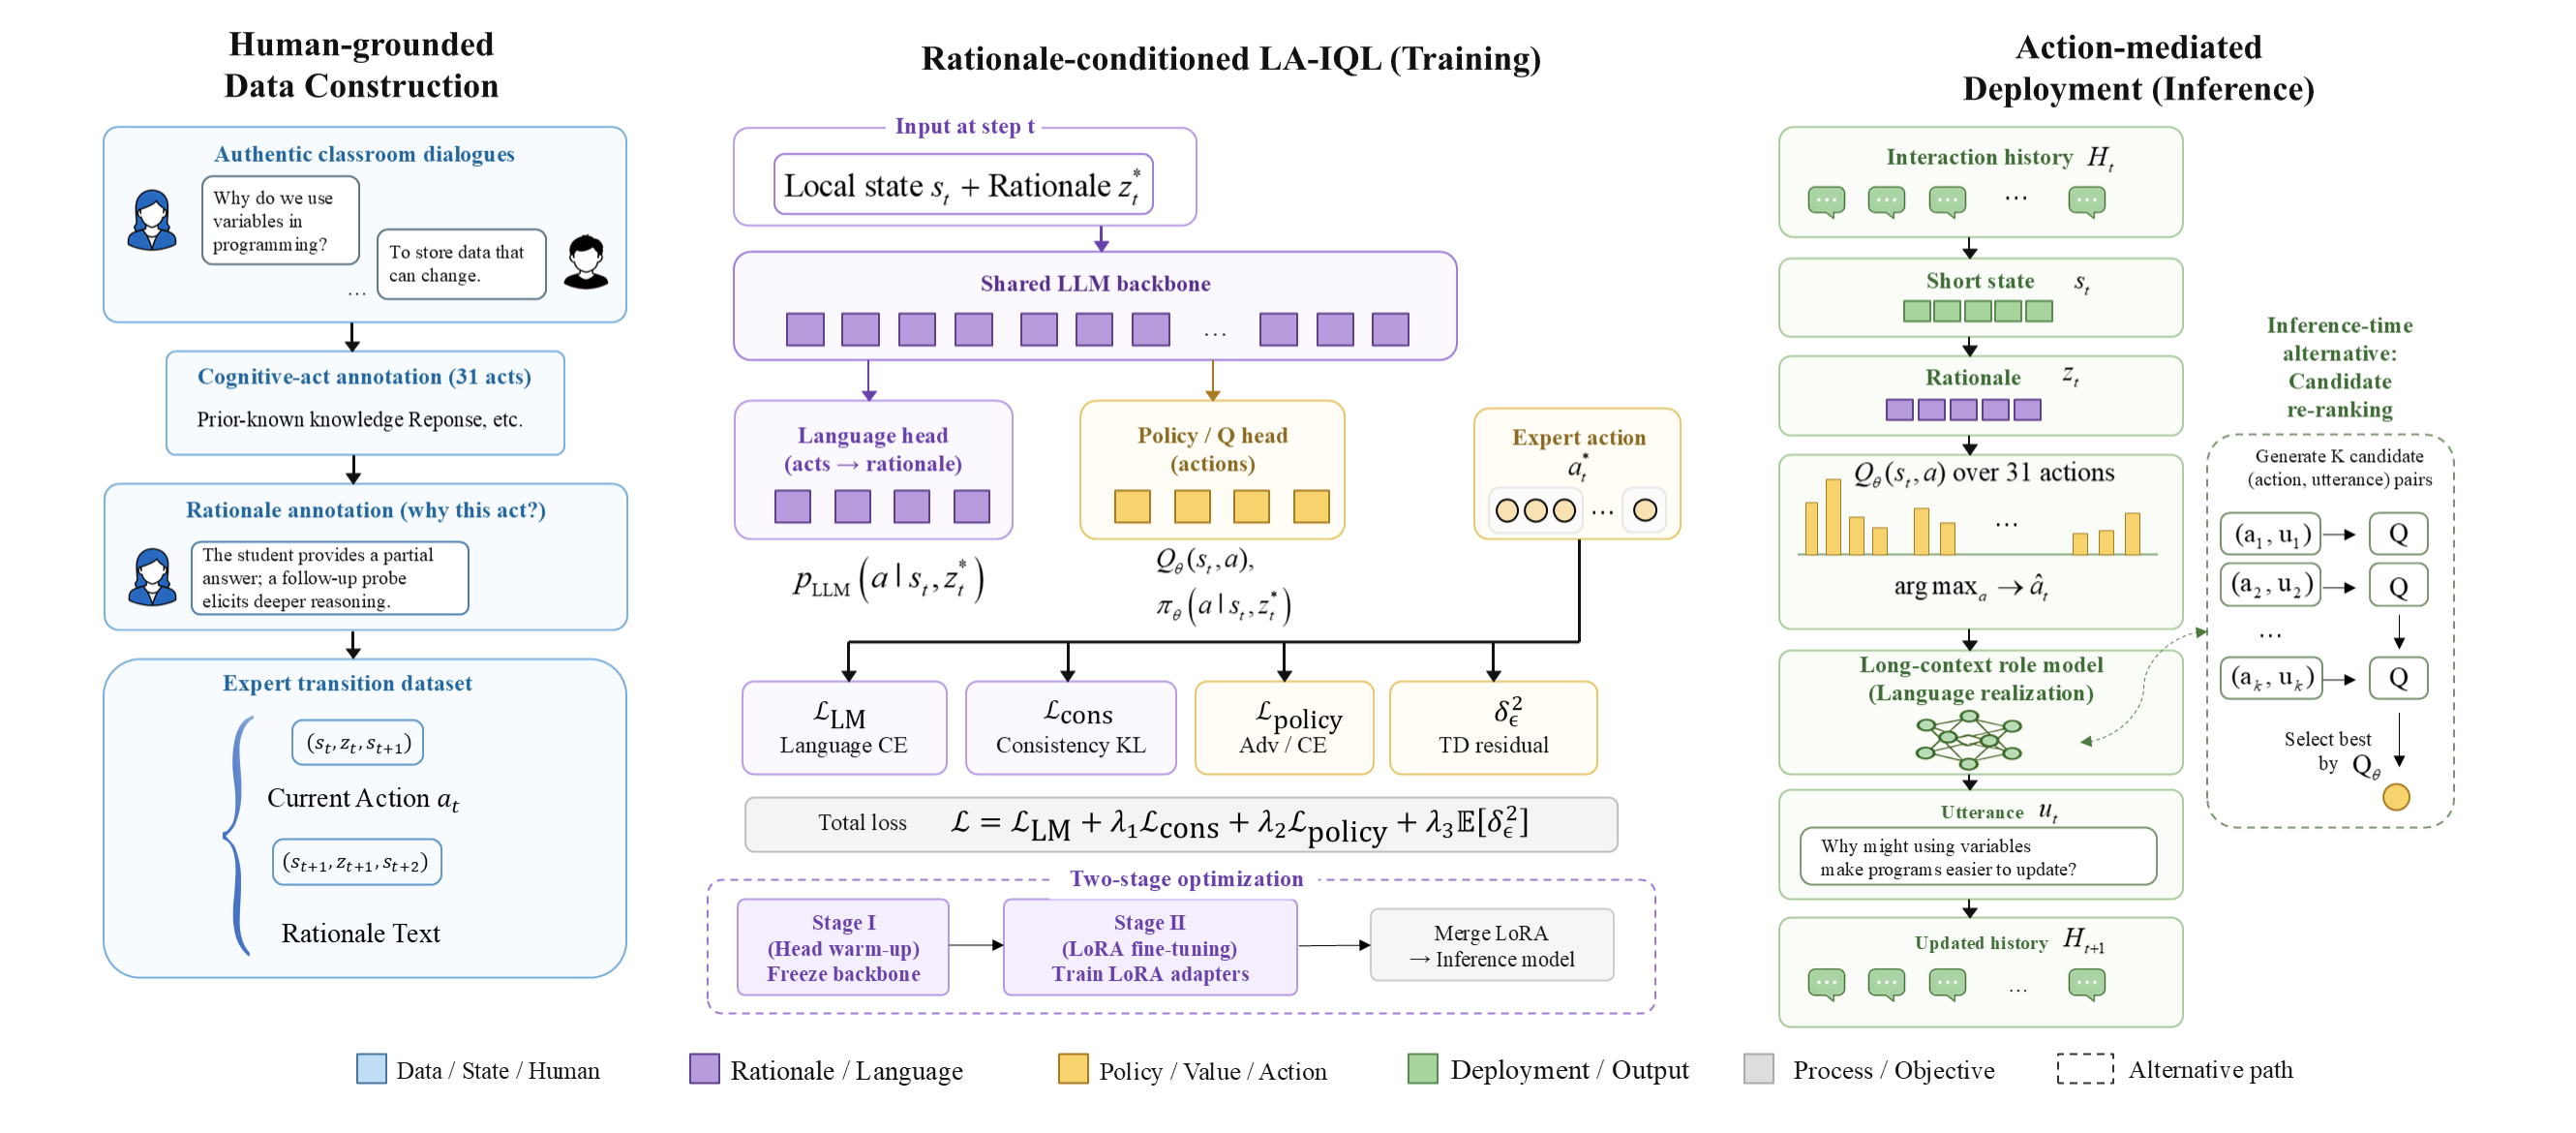
\includegraphics[width=\textwidth]{figure/LA-IQL-framework.png}
  \caption{\textbf{LA-IQL framework and technical flow.}
  Human-grounded classroom dialogue and cognitive-act annotations are converted
  into rationale-augmented expert transitions (left). Rationale-conditioned
  LA-IQL jointly trains language and policy/value components with language,
  consistency, policy, and temporal-difference objectives (center). At
  inference, the learned policy selects an interaction action and a long-context
  role model realizes it as an utterance; candidate re-ranking is shown as an
  inference-time alternative (right).}
  \Description{A three-part framework diagram. The left section constructs an
  expert transition dataset from authentic classroom dialogue, cognitive-act
  labels, and rationale annotations. The center section shows a shared language
  model with language and policy heads, four training objectives, and three-stage
  optimization. The right section shows interaction history, short state,
  rationale, action-value selection, long-context language realization,
  utterance generation, and an optional candidate re-ranking branch.}
  \label{fig:method-overview}
\end{figure*}
 
The role model is recorded as \texttt{deepseek-chat} for both teacher and
student roles. It uses a long window of 30 dialogue turns and five action steps;
where sampling applies, it uses a temperature of $0.8$ and top-$p$ of 1. The
artifact retains the mutable API alias rather than an immutable model snapshot.
In the reported evaluation, generation stops at \texttt{END} or the 100-action horizon.

We additionally explored candidate re-ranking as an inference-time adjustment. The role model samples six action--utterance candidates in a fixed schema---three for the teacher and three for the student---and thereby induces $q_\phi(\mathcal C_t\mid h_t)$ over $\mathcal{C}_t=\{(a_{t,j},u_{t,j})\}_{j=1}^{6}$. The selected index is
\begin{equation}
\begin{aligned}
j^*&=\arg\max_{1\leq j\leq 6}Q_\theta(s_t,z_t,a_{t,j}),\\
(a_t,u_t)&=(a_{t,j^*},u_{t,j^*}).
\end{aligned}
\label{eq:proposal-constrained-selection}
\end{equation}
This adjustment scores a candidate through its associated action label and does not directly score $u_{t,j}$; candidates sharing an action are therefore indistinguishable to $Q_\theta$, and ties retain proposal order. It is proposal-constrained because an action cannot be selected unless it appears in $\mathcal C_t$. Unlike default direct decoding, the role model therefore controls action support while the value model only chooses among proposed actions.

\section{Experimental Design}
\label{sec:experiments}

\paragraph{Research questions.}
We answer four research questions. Together, they test whether an interactive
agent's explicit strategy layer is human-pattern-aligned, temporally organized,
context-sensitive, and legibly realized:
\begin{enumerate}[label=\textbf{RQ\arabic*:},leftmargin=*,itemsep=2pt,topsep=2pt,parsep=0pt]
\item How do action-mediated learned policies compare with direct
language generation and statistical policies in behavioral diversity,
repetition, and alignment with held-out patterns from authentic human
interaction?
\item What long-horizon behavioral differences are observed between
the evaluated fixed checkpoints with and without temporal-difference
regularization, and between direct full-action-space selection and
proposal-constrained candidate re-ranking under the completed configurations?
\item Do generated rationales contain action-relevant information beyond the
dialogue state and explicit label leakage?
\item How are differences in interaction-strategy selection reflected in the
introduction, connection, and development of expressed knowledge over
long-horizon dialogue?
\end{enumerate}

These questions primarily target model- and trajectory-level structural
properties. Participant judgments are not used as evidence of educational
effectiveness; we add a supplementary excerpt-level evaluation to examine
whether differences between LA-IQL and direct language generation are
perceptible in interactional variety, resemblance to teacher--student
interaction, and support for understanding and discussion.

\subsection{Data and Splits}

The source classroom recordings were obtained from China's National Public
Service Platform for Educational Resources\footnote{\url{https://www.eduyun.cn}},
a national platform supported by the Ministry of Education. The platform hosts
K--12 lessons contributed voluntarily by teachers using classroom recording
systems and covers schools across major provinces and municipalities in China.
We selected lessons from this source because of its broad geographic and
subject coverage, institutional provenance, and publicly accessible materials,
which facilitate inspection of the source lessons. From the resulting classroom
corpus described in Section~\ref{sec:problem}, we use 50 lessons in this study.
Each source turn retains its previously assigned cognitive-act label and
recorded speaker role. We pair these two fields and add the role-independent
\texttt{END} action to construct the 31 interaction acts and transition tuples
used by LA-IQL.
We use a frozen, stratified lesson-level split of 35 training, five validation,
and 10 test lessons rather than splitting by dialogue turn, so
that windows from the same classroom session cannot occur in both partitions.
The split is stratified by subject and school stage; lesson identifiers are
disjoint across all three partitions, and two lessons used in pilot
smoke tests are excluded from the test partition.  The split manifest, random
seed, data hash, and split-level action frequencies are recorded before formal
evaluation.  The same test lessons were inspected in an earlier
horizon-20 run; we disclose this prior access and do not alter test membership
for the horizon-100 baseline evaluation reported below.

\begin{table}[t]
\centering
\small
\begin{tabularx}{\columnwidth}{@{}>{\raggedright\arraybackslash}p{0.27\columnwidth}>{\raggedright\arraybackslash}X@{}}
\toprule
Component & Recorded configuration \\
\midrule
Policy model & \texttt{Qwen/Qwen3.5-0.8B}; 31-action rationale-conditioned dual head \\
Rationale annotation & \texttt{deepseek-chat}; temperature 0.7; 9,168 rewritten non-END records; 201 END transitions omitted \\
Role realization & \texttt{deepseek-chat}; temperature 0.8; top-$p$ 1; 30-turn/5-action context \\
Policy observation & Two dialogue turns and two action labels; max input length 512; rationale budget 256 tokens \\
Formal split & 35/5/10 lessons; subject--stage stratification; split seed 20260731 \\
Rollout & 10 test lessons; horizon 100; \texttt{END} disabled before step 50; margin 3.0 \\
Randomness & Full/no-TD: one checkpoint each, generation seeds 42--44; BC: independent train/gen. seeds 42--44 \\
\bottomrule
\end{tabularx}
\caption{Implementation summary. Values are transcribed from checkpoint,
split, annotation, and formal-trajectory artifacts. Historical training fields
not retained by those artifacts are documented as unavailable in
Appendix~\ref{sec:reproducibility}.}
\label{tab:implementation-summary}
\end{table}

\subsection{Baselines, Controls, and System Comparisons}
\label{sec:comparison-roles}

Our comparisons have four distinct roles and should not be read as one set of
exchangeable baselines.

\paragraph{Generation baselines.}
Direct role-conditioned generation and a constrained teacher prompt test what
end-to-end prompted generation produces without a separately learned action
policy. They provide output-level references, not component-matched ablations
of LA-IQL.

\paragraph{Learned-policy comparisons.}
Frozen BC and LoRA BC are supervised next-action predictors trained on the same
31-action space and source split. Frozen BC trains only a 31-way classification
head over a frozen \texttt{Qwen/Qwen3.5-0.8B} backbone; LoRA BC adapts the same
backbone with LoRA under the same next-action cross-entropy objective. Neither
uses rationales, a TD objective, inverse Q-learning, or Q-value decoding. Both
use three independently trained checkpoints and realize selected actions with
the same role model and formal horizon-100 rollout protocol. They test how the
implemented one-step supervised policy family behaves under the shared action
interface; because several training components differ together, BC--LA-IQL
differences do not isolate any single LA-IQL component.

\paragraph{Statistical diagnostic controls.}
Uniform action sampling, expert-frequency sampling, and a first-order Markov
policy isolate distributional and sequential statistics. They are not learned,
state-conditioned interactive policies and are not candidates for overall
system superiority. In particular, the Markov control estimates
$p(a_t\mid a_{t-1})$ from the frozen training split. It is deliberately well
matched to bigram- and transition-based alignment measures, but it does not observe
dialogue content, the current instructional state, or a rationale, and it
does not produce an utterance whose realization can be inspected. Its role is
therefore to test how much local human-pattern alignment can be recovered from
aggregate action transitions alone.

\paragraph{Inference-time system comparison.}
LA-IQL uses the direct decoding rule in
Equation~\ref{eq:direct-policy-decoding}. \emph{LA-IQL + candidate re-ranking}
uses the same learned policy checkpoint but substitutes the proposal-constrained
rule in Equation~\ref{eq:proposal-constrained-selection}; it is therefore an
inference-time system configuration, not a separately trained baseline. This
comparison was elevated after inspection of the current held-out results and is
descriptive rather than a preregistered model-selection claim. Both
configurations use the same checkpoint, lessons, horizon, role-model
temperature, and generation seeds. However, Direct uses rationale temperature
0.0 whereas Candidate uses 0.6, so their differences characterize the completed
systems and cannot be attributed solely to candidate re-ranking.

\paragraph{TD checkpoint contrast.}
To examine the checkpoint-level difference associated with temporal-difference
regularization, we add \emph{LA-IQL w/o TD (Direct)}, trained with Stage~3 TD
weight 0 rather than 1. It uses Direct decoding, rationale temperature 0.0,
the same held-out lessons, role model, context windows, generation seeds,
horizon, and stopping rule as the main LA-IQL system. The recovered training
fields otherwise match (Appendix~\ref{sec:reproducibility}), but each condition
contains one trained checkpoint; we therefore treat this as a fixed-checkpoint
contrast rather than a training-seed-general causal estimate.

\subsection{Evaluation Metrics}

For interaction-pattern diversity, the main analysis reports action Distinct-2, two-step cycle rate, empirical action entropy, and expert-pattern coverage, capturing local variety, repetitive degeneration, distributional diversity, and expert-supported breadth, respectively.
For expert-pattern alignment, we use Jensen--Shannon divergence between generated and expert action patterns, transition-matrix distance, and expert support for generated action $n$-grams. These are behavioral-distribution measures, not tests of whether an action is contextually appropriate for the dialogue state. Their overlap with the Markov control's inductive bias makes that control a demanding local-pattern reference rather than evidence of state-sensitive interaction competence.
For rationale--action consistency (RQ3), we mask deterministic label strings and train an independent 31-way action predictor on disjoint lessons using the state, the rationale, or both.
Our principal automatic measure is incremental simulatability:
\begin{equation}
\Delta_{\mathrm{sim}}
=
F_{1}^{\mathrm{macro}}(s_t,z_t\!\rightarrow\!a_t)
-
F_{1}^{\mathrm{macro}}(s_t\!\rightarrow\!a_t),
\label{eq:g3-simulatability}
\end{equation}
where the target is the evaluated system's selected action.
We also report masked rationale-only Macro-F1, majority, leakage, and shuffled-rationale controls. Predictability alone does not establish causal faithfulness~\citep{hase2020leakage,jacovi2020faithfully}; we therefore describe RQ3 as a simulatability diagnostic rather than an explanation-quality measure.
For secondary language-realization diagnostics, we report redundancy and
rule-defined severe violations. This deliberately narrow diagnostic set does
not measure contextual or classroom appropriateness; open-ended text overlap is
secondary because multiple responses can be valid.
For RQ4, each system--generation-seed--lesson trajectory is a measurement
unit. Repeated runs are averaged within each system--lesson unit before
paired comparisons; the held-out lesson is the unit of statistical inference
and cluster resampling. Its primary evidence
is an evidence-grounded knowledge-graph extraction followed by deterministic
calculation of three prespecified endpoints: unique entities per 100 non-END
turns, mean relational degree, and the proportion of final relations first
introduced in the latter half of a trajectory. Rule-based diagnostics provide
auditable anchors. We report the knowledge-graph endpoints without combining
them into a classroom-quality score.
Appendix~\ref{sec:evaluation-details} gives the complete metric and intervention protocol.

\subsection{Evaluation Protocol}

Action-pattern Jensen--Shannon divergence is the primary alignment endpoint.
Diversity and alignment jointly address cross-system comparisons (RQ1) and
checkpoint and inference-configuration comparisons (RQ2).
The reported trajectory results cover seeds 42--44 and 10 frozen test lessons
per seed at horizon 100. For the LA-IQL configurations and generation controls,
these are three stochastic rollouts from a fixed checkpoint or inference
procedure. For Frozen BC and LoRA BC, each seed identifies an independently
trained checkpoint and its matching generation run. We report mean $\pm$
population standard deviation across seed aggregates; the BC variation thus
combines training and generation variation, whereas the LA-IQL variation does
not include training-seed uncertainty. For
learned-system comparisons, we additionally pair the 30 matching
generation-seed--lesson trajectories, cluster resampling by the 10 lessons, run
10,000 bootstrap resamples, and report percentile 95\% intervals. The reported
TD $p$-values are unadjusted within an exploratory matched-checkpoint family;
the Direct--Candidate table applies Benjamini--Hochberg correction over its 10
retained comparisons. The TD contrast holds Direct decoding and rationale
temperature fixed. By contrast, Direct and Candidate differ in rationale
temperature and were examined after observing held-out results, so that
comparison remains a descriptive system-level contrast rather than a
confirmatory causal decoding effect.

\paragraph{Supplementary human evaluation.}
Thirty-five adult volunteers completed the shortened questionnaire; two records
contained no excerpt ratings, leaving 33 complete responses (25 women and eight
men). Each participant independently rated six blinded, same-topic excerpt sets
on three five-point items: interactional variety, resemblance to authentic
teacher--student interaction, and support for understanding and discussion.
For the reported model comparison, we aggregate the six LA-IQL Direct and six
Direct-role LLM ratings within participant and dimension, apply paired Wilcoxon
signed-rank tests, and use Holm correction across the three dimensions. Because
removing four sets from the longer instrument left source positions unbalanced,
we additionally fit a sensitivity model with participant, item, dimension, and
display-position effects and participant-clustered standard errors. The
questionnaire also collected ratings for authentic transcript excerpts, but
unavoidable transcription loss and differences in excerpt length and exact
dialogue state made those scores non-equivalent to the generated excerpts. We
therefore exclude that reference condition from model-comparison inference and
treat this evaluation as supplementary and exploratory.

Table~\ref{tab:g1-core-results} reports cross-system diversity results (RQ1).

\begin{table*}[t]
\centering
\small
\setlength{\tabcolsep}{4pt}
\resizebox{\textwidth}{!}{\begin{tabular}{lrrrr}
\toprule
System or control & Dist.-2 $\uparrow$ & Cycle-2 $\downarrow$ & $H_{\mathrm{norm}}$ $\uparrow$ & Cov.@20 $\uparrow$ \\
\midrule
\multicolumn{5}{l}{\emph{Generation baselines}} \\
Direct Role LLM & $0.4364 \pm 0.0348$ & $0.0286 \pm 0.0088$ & $0.6722 \pm 0.0102$ & $0.5500 \pm 0.0408$ \\
Constrained Prompt & $0.5279 \pm 0.0117$ & $0.1520 \pm 0.0147$ & $0.6818 \pm 0.0015$ & $0.5333 \pm 0.0236$ \\
\addlinespace
\multicolumn{5}{l}{\emph{Statistical diagnostic controls}} \\
Uniform Random & $0.9593 \pm 0.0048$ & $0.0000 \pm 0.0000$ & $0.9287 \pm 0.0066$ & $0.3500 \pm 0.0000$ \\
Expert Frequency & $0.6951 \pm 0.0277$ & $0.0067 \pm 0.0033$ & $0.7144 \pm 0.0111$ & $0.9500 \pm 0.0000$ \\
First-order Markov & $0.5144 \pm 0.0072$ & $0.0819 \pm 0.0140$ & $0.7072 \pm 0.0012$ & $1.0000 \pm 0.0000$ \\
\addlinespace
\multicolumn{5}{l}{\emph{Learned-policy comparisons}} \\
Frozen BC & $0.0694 \pm 0.0062$ & $0.0072 \pm 0.0069$ & $0.2379 \pm 0.0134$ & $0.3167 \pm 0.1434$ \\
LoRA BC & $0.0539 \pm 0.0267$ & $\mathbf{0.0017 \pm 0.0013}$ & $0.1267 \pm 0.0940$ & $0.3333 \pm 0.2055$ \\
\addlinespace
\multicolumn{5}{l}{\emph{LA-IQL checkpoint and inference configurations}} \\
LA-IQL w/o TD (Direct) & $0.4118 \pm 0.0236$ & $0.2607 \pm 0.0193$ & $0.6412 \pm 0.0120$ & $\mathbf{1.0000 \pm 0.0000}$ \\
\textbf{LA-IQL} & $0.4370 \pm 0.0101$ & $0.1708 \pm 0.0126$ & $\mathbf{0.6670 \pm 0.0084}$ & $\mathbf{1.0000 \pm 0.0000}$ \\
LA-IQL + candidate re-ranking & $\mathbf{0.4478 \pm 0.0205}$ & $\mathbf{0.0488 \pm 0.0013}$ & $0.6664 \pm 0.0131$ & $0.7000 \pm 0.0408$ \\
\bottomrule
\end{tabular}
}
\caption{Cross-system diversity results for RQ1 (mean $\pm$ population SD over three completed runs).
Row groups denote different evidential roles rather than a single
fairness-matched ranking. Bold values are restricted to the learned-policy and
LA-IQL configuration rows and do not imply cross-category system superiority.
Metrics must be interpreted jointly because low Cycle-2 alone does not exclude
other forms of recurrence.}
\label{tab:g1-core-results}
\end{table*}

Table~\ref{tab:g2-baseline-results} reports cross-system alignment results (RQ1) on the same runs. Paired JS uses the frozen $31^2$ bigram vocabulary and Jeffreys smoothing ($\alpha=0.5$); transition JS weights rows by expert frequency, and support uses training-split $n$-grams.

\begin{table*}[t]
\centering
\small
\setlength{\tabcolsep}{4pt}
\resizebox{\textwidth}{!}{\begin{tabular}{lrrrrr}
\toprule
System or control & Paired bigram JS $\downarrow$ & Pooled bigram JS $\downarrow$ & Transition JS $\downarrow$ & Bigram support $\uparrow$ & Trigram support $\uparrow$ \\
\midrule
\multicolumn{6}{l}{\emph{Generation baselines}} \\
Direct Role LLM & $0.1030 \pm 0.0013$ & $0.3423 \pm 0.0184$ & $0.1708 \pm 0.0049$ & $0.7532 \pm 0.0167$ & $0.4250 \pm 0.0267$ \\
Constrained Prompt & $0.1096 \pm 0.0016$ & $0.3795 \pm 0.0072$ & $0.1880 \pm 0.0069$ & $0.9218 \pm 0.0092$ & $0.4731 \pm 0.0144$ \\
\addlinespace
\multicolumn{6}{l}{\emph{Statistical diagnostic controls}} \\
Uniform Random & $0.1235 \pm 0.0012$ & $0.4661 \pm 0.0042$ & $0.2293 \pm 0.0028$ & $0.4105 \pm 0.0249$ & $0.0431 \pm 0.0047$ \\
Expert Frequency & $0.1036 \pm 0.0006$ & $0.2868 \pm 0.0036$ & $0.1995 \pm 0.0036$ & $0.8125 \pm 0.0161$ & $0.3316 \pm 0.0032$ \\
First-order Markov & $0.0791 \pm 0.0009$ & $0.0982 \pm 0.0038$ & $0.1249 \pm 0.0017$ & $0.9935 \pm 0.0021$ & $0.8557 \pm 0.0169$ \\
\addlinespace
\multicolumn{6}{l}{\emph{Learned-policy comparisons}} \\
Frozen BC & $0.1607 \pm 0.0075$ & $0.5807 \pm 0.0347$ & $0.3053 \pm 0.0166$ & $\mathbf{0.9983 \pm 0.0017}$ & $0.7412 \pm 0.2445$ \\
LoRA BC & $0.1674 \pm 0.0057$ & $0.6041 \pm 0.0309$ & $0.2811 \pm 0.0255$ & $0.9949 \pm 0.0071$ & $\mathbf{0.9143 \pm 0.0847}$ \\
\addlinespace
\multicolumn{6}{l}{\emph{LA-IQL checkpoint and inference configurations}} \\
LA-IQL w/o TD (Direct) & $0.0835 \pm 0.0022$ & $\mathbf{0.1530 \pm 0.0177}$ & $0.1308 \pm 0.0041$ & $0.9833 \pm 0.0005$ & $0.8773 \pm 0.0125$ \\
\textbf{LA-IQL} & $\mathbf{0.0827 \pm 0.0031}$ & $0.1637 \pm 0.0085$ & $\mathbf{0.1299 \pm 0.0050}$ & $0.9906 \pm 0.0024$ & $0.8772 \pm 0.0064$ \\
LA-IQL + candidate re-ranking & $0.1059 \pm 0.0025$ & $0.3116 \pm 0.0132$ & $0.1648 \pm 0.0035$ & $0.9522 \pm 0.0045$ & $0.4874 \pm 0.0063$ \\
\bottomrule
\end{tabular}
}
\caption{Cross-system expert-pattern alignment for RQ1 (mean $\pm$ population SD over three
completed runs).
Row groups have the distinct evidential roles defined in
Section~\ref{sec:comparison-roles}; bold is restricted to learned-policy and LA-IQL
configuration rows. The first-order Markov control
directly models the local transitions measured by several columns but does not
condition on dialogue content.}
\label{tab:g2-baseline-results}
\end{table*}

\subsection{Experimental Results}

\paragraph{The evaluated TD checkpoint shows less repetitive long-horizon organization.}
Table~\ref{tab:td-ablation-paired} reports the matched Direct-decoding
checkpoint contrast. The w/o-TD checkpoint has more two-step cycles
($0.2607$ vs. $0.1708$; TD--w/o-TD difference $-0.0900$, 95\% CI
$[-0.1400,-0.0438]$,
$p=.0002$) and greater motif recurrence ($0.5379$ vs. $0.3957$; difference
$-0.1422$, 95\% CI $[-0.2013,-0.0889]$, $p=.0002$). Relative to the
TD-regularized checkpoint, these correspond to 53\% more two-step cycles and
36\% more repeated motifs for the w/o-TD checkpoint. Distinct-2 and normalized
entropy are numerically higher with TD but do not differ reliably. Both
systems cover all top-20 expert patterns, supporting the interpretation that,
for these checkpoints, lower recurrence does not coincide with abandoning
those common patterns.

Local expert-distribution alignment changes little. Paired bigram JSD is
$0.0827$ with TD and $0.0835$ without TD (difference $-0.0007$, 95\% CI
$[-0.0063,0.0043]$, $p=.8281$); transition JSD is likewise
not reliably different. Bigram support shows a borderline descriptive advantage for
TD ($0.9906$ vs. $0.9833$, $p=.0510$). For these fixed checkpoints, the
observed TD-associated difference is concentrated in recurrent sequence
structure rather than local imitation fidelity. Our inference is therefore
explicitly bounded to the evaluated checkpoints rather than the training
objective across random initializations.

\paragraph{The implemented one-step BC policies exhibit narrow recurrent patterns.}
The two supervised BC systems provide learned-policy references rather than
single-component ablations. In the completed runs, Frozen BC and LoRA BC obtain
Distinct-2 values of $0.0694$ and
$0.0539$, normalized entropies of $0.2379$ and $0.1267$, and repeated-motif
rates of $0.9690$ and $0.9697$, respectively. Direct LA-IQL is substantially
more diverse and less motif-recurrent on the same endpoints (Distinct-2
$0.4370$, normalized entropy $0.6670$, and motif rate $0.3957$). The BC
Cycle-2 rates are low, but this does not indicate broad temporal organization:
their near-unit motif rates show that they predominantly repeat a narrow set of
local patterns rather than alternate in the specific two-step form measured by
Cycle-2. The complete recurrence results appear in
Table~\ref{tab:appendix-full-g1-results}.

The same baselines also reproduce training-supported local transitions without
matching the held-out distribution closely. Frozen BC and LoRA BC reach bigram
support of $0.9983$ and $0.9949$, but their paired bigram JSD values are
$0.1607$ and $0.1674$, compared with $0.0827$ for Direct LA-IQL. LoRA BC has
higher trigram support ($0.9143$ vs. $0.8772$), illustrating why support must be
read jointly with distributional divergence and recurrence. These descriptive
comparisons show that, for these implemented BC configurations, high local
support does not coincide with diverse or expert-distribution-aligned
long-horizon organization. They do not isolate rationales, TD regularization,
or Q-value decoding as the sole cause of the difference.

\begin{table*}[t]
\centering
\small
\setlength{\tabcolsep}{4pt}
\begin{tabular}{llrrr}
\toprule
Metric family & Paired metric (TD $-$ w/o TD) & Difference & 95\% CI & $p$ \\
\midrule
Diversity & Distinct-2 $\uparrow$ & $+0.0252$ & $[-0.0282,\ 0.0688]$ & $0.3186$ \\
Diversity & Cycle-2 $\downarrow$ & $-0.0900$ & $[-0.1400,\ -0.0438]$ & $0.0002$ \\
Diversity & Motif rate $\downarrow$ & $-0.1422$ & $[-0.2013,\ -0.0889]$ & $0.0002$ \\
Diversity & Normalized entropy $\uparrow$ & $+0.0258$ & $[-0.0156,\ 0.0659]$ & $0.2204$ \\
Alignment & Paired bigram JSD $\downarrow$ & $-0.0007$ & $[-0.0063,\ 0.0043]$ & $0.8281$ \\
Alignment & Transition JSD $\downarrow$ & $-0.0009$ & $[-0.0091,\ 0.0055]$ & $0.8581$ \\
Alignment & Bigram support $\uparrow$ & $+0.0073$ & $[-0.00001,\ 0.0140]$ & $0.0510$ \\
Secondary & Local trigram redundancy $\downarrow$ & $-0.00001$ & $[-0.0042,\ 0.0041]$ & --- \\
\bottomrule
\end{tabular}
\caption{Fixed-checkpoint temporal-difference contrast under Direct decoding. Values
compare LA-IQL with and without the TD term over the same 30 generation-seed--lesson
trajectories, clustered by 10 held-out lessons, with 10,000 bootstrap
resamples. Both systems use rationale temperature 0.0 and otherwise identical
generation settings. Positive differences mean the TD model is numerically
larger; metric arrows indicate the desirable direction.}
\label{tab:td-ablation-paired}
\end{table*}
 
\paragraph{Local transition statistics form a strong but limited reference.}
Tables~\ref{tab:g1-core-results} and~\ref{tab:g2-baseline-results} report the
formal trajectory measurements. The first-order Markov control obtains the
lowest paired bigram JSD ($0.0791$), pooled bigram JSD ($0.0982$), and
transition-row JSD ($0.1249$), compared with $0.0827$, $0.1637$, and $0.1299$
for Direct LA-IQL. It also reaches $0.9935$ bigram support, while Direct
LA-IQL is higher on trigram support ($0.8772$ vs. $0.8557$).

This result follows from a substantive match between model and measurement:
the control estimates $p(a_t\mid a_{t-1})$ from training trajectories, while
bigram JSD and transition-row JSD measure the corresponding local action
structure. High support and coverage can likewise arise from conservatively
resampling training-supported transitions. These are legitimate strengths on
the stated alignment endpoints, not an error to discount. However, the control never
observes the dialogue text or instructional state and cannot expose whether a
locally frequent transition is appropriate in context. We therefore interpret
it as evidence that local human-pattern reproduction is achievable with a
simple sequential statistic, and not as evidence that the Markov policy is a
more capable interactive agent. This distinction motivates reporting alignment
alongside state-conditioned decision traces, repetition diagnostics, and
action--utterance realization checks.

\paragraph{A frozen intervention provides exploratory evidence of text sensitivity.}
We evaluated the main Full checkpoint on five pre-existing, evenly spaced
states from each of the 10 held-out lessons ($N=50$). Within each lesson, a
cyclic donor replaced utterance semantics while preserving the speaker
sequence, number of utterances, and action history. Relative to the original
states, the probability assigned to the expert action decreased by $0.0767$
(lesson-cluster bootstrap 95\% CI $[0.0153,0.1288]$), 60\% of argmax actions
flipped (CI $[0.48,0.72]$), and mean policy JSD was $0.2957$ (CI
$[0.2476,0.3431]$). The 31-class Macro-F1 decrease was $0.0201$, with an
interval crossing zero ($[-0.0185,0.0649]$). This intervention indicates that
the fixed policy distribution responds to dialogue text beyond the preserved
action history. Its small sample, deterministic donor construction, and lack of
human judgments mean it does not establish that the response is contextually
appropriate. Appendix~\ref{sec:context-intervention} records the protocol.

\paragraph{Candidate re-ranking changes the inference-time control trade-off.}
Direct LA-IQL is closer to the held-out expert
distribution than Candidate: paired bigram JSD is $0.0827$ versus $0.1059$,
and training-expert bigram support is $0.9906$ versus $0.9522$. Across 30
matched generation-seed--lesson units, the Direct--Candidate difference in bigram JSD is
$-0.0232$, 95\% CI $[-0.0305,-0.0152]$, BH-adjusted $q<.0001$.

This alignment does not imply uniformly better interaction dynamics. Direct
has substantially more two-step cycles ($0.1708$ vs. $0.0488$; paired
difference $+0.1220$, 95\% CI $[0.0986,0.1447]$, $q<.0001$) and repeated
motifs ($0.3957$ vs. $0.1413$; difference $+0.2543$, 95\% CI
$[0.2100,0.2963]$, $q<.0001$). Distinct-2 has no reliable paired difference
($-0.0108$, 95\% CI $[-0.0377,0.0165]$, $q=.5483$). The completed
configurations therefore differ more clearly in action-sequence organization
than in local combinatorial diversity. Because Candidate reuses the Direct
policy checkpoint and also changes rationale temperature, this is a comparison
of two inference-time systems, not evidence that a separately learned Candidate
policy is superior or an isolated ablation of re-ranking.

\begin{table*}[t]
\centering
\small
\setlength{\tabcolsep}{4pt}
\begin{tabular}{llrrr}
\toprule
Metric family & Paired metric (Direct $-$ Candidate) & Difference & 95\% CI & BH $q$ \\
\midrule
Diversity & Distinct-2 $\uparrow$ & $-0.0108$ & $[-0.0377,\ 0.0165]$ & $0.5483$ \\
Diversity & Cycle-2 $\downarrow$ & $+0.1220$ & $[0.0986,\ 0.1447]$ & $<.0001$ \\
Diversity & Motif rate $\downarrow$ & $+0.2543$ & $[0.2100,\ 0.2963]$ & $<.0001$ \\
Alignment & Paired bigram JSD $\downarrow$ & $-0.0232$ & $[-0.0305,\ -0.0152]$ & $<.0001$ \\
Alignment & Bigram support $\uparrow$ & $+0.0384$ & $[0.0283,\ 0.0492]$ & $<.0001$ \\
Alignment & Trigram support $\uparrow$ & $+0.3898$ & $[0.3551,\ 0.4238]$ & $<.0001$ \\
\bottomrule
\end{tabular}
\caption{Paired Direct--Candidate comparison over 30 matched generation-seed--lesson
units (10,000 bootstrap resamples; percentile intervals; BH correction over
10 retained comparisons). Positive values mean Direct is numerically larger; metric
arrows indicate the desirable direction. The configurations also differ in
rationale temperature, so this is a system-level comparison rather than a
single-factor decoding ablation.}
\label{tab:direct-candidate-paired}
\end{table*}

\paragraph{A rule-selected trace makes the recurrence difference inspectable.}
Before reading trajectory text, we selected the matched lesson--seed unit with
the largest Direct--Candidate Cycle-2 difference, breaking any tie by motif-rate
difference and then lexical order. This rule selects the Grade-9 chemistry
lesson on atomic structure at generation seed 43 (Cycle-2: $0.309$ vs.
$0.052$; motif rate: $0.55$ vs. $0.17$). Table~\ref{tab:trajectory-example}
shows the earliest four-turn Direct cycle and the same turn positions in the
matched Candidate trajectory. Rationales and utterances are abridged
translations from Chinese; action symbols follow Table~\ref{tab:action-space}.

\begin{table*}[t]
\centering
\footnotesize
\begin{tabularx}{\textwidth}{@{}>{\raggedright\arraybackslash}p{0.12\textwidth}>{\raggedright\arraybackslash}X@{}}
\toprule
Configuration and local context & Four-turn decision trace: action; rationale $\rightarrow$ utterance \\
\midrule
Direct\\
Student had just restated the teacher's explanation of nuclear force.
& \textbf{t13 Teacher--Ag:} confirm understanding and extend the issue $\rightarrow$
``Exactly. Does having more protons mean stronger nuclear force and a more stable nucleus?''
\newline \textbf{t14 Student--Pk:} answer the hypothesis from prior knowledge $\rightarrow$
``I think so; more protons should mean more nuclear force.''
\newline \textbf{t15 Teacher--Ag:} affirm the analogy, then introduce a competing force $\rightarrow$
``But electrostatic repulsion also increases; which force wins?''
\newline \textbf{t16 Student--Pk:} respond to that comparison $\rightarrow$
``Repulsion also grows, so the nucleus may not necessarily become more stable.'' \\
\addlinespace
Candidate\\
Student had just estimated electron mass and located most atomic mass in the nucleus.
& \textbf{t13 Teacher--Gu:} confirm the estimate and consolidate mass-distribution understanding $\rightarrow$
``Draw an atomic model and mark each part's position and approximate mass share.''
\newline \textbf{t14 Student--An:} construct and explain the requested model $\rightarrow$
``A small central nucleus contains protons and neutrons; light electrons move outside it.''
\newline \textbf{t15 Teacher--Iu:} refine the diagram's component placement and mass analogy $\rightarrow$
``What force keeps the electrons and nucleus in a stable relation?''
\newline \textbf{t16 Student--Pk:} supply the requested relation $\rightarrow$
``The attraction between negative electrons and the positive nucleus.'' \\
\bottomrule
\end{tabularx}
\caption{Rule-selected inspectable case from formal trajectories (lesson 4873,
generation seed 43, turns 13--16). The Direct window instantiates an
Ag--Pk--Ag--Pk two-step cycle, whereas Candidate traverses Gu--An--Iu--Pk.
The entries preserve the recorded action, rationale intent, and utterance
content while abbreviating the original text for space.}
\label{tab:trajectory-example}
\end{table*}

The action trace exposes recurring decision types that would be difficult to
audit from surface text alone. At the same time, the Direct utterances advance
from a claim about nuclear force to the countervailing role of electrostatic
repulsion. The Candidate trace also exposes a local rationale--realization shift
at t15: the recorded rationale focuses on refining placement and mass, while
the utterance asks about electrostatic stability. The example therefore
illustrates, but does not by itself validate, the aggregate recurrence contrast
or realization quality: a repeated action motif is not equivalent to verbatim
repetition or instructional failure. We consequently use the case for
structural interpretation rather than a human-preference ranking.

 
\paragraph{Rationales carry action-predictive information.}
Under the same RQ3 dual TF--IDF evaluator, masked rationale-only Macro-F1 is
$0.3986$ for Direct and $0.1013$ for Candidate, compared with state-only
scores of $0.0159$ and $0.0123$. Run-level incremental simulatability
$\Delta_{\mathrm{sim}}$ is $0.3885$ for Direct and $0.0863$ for Candidate.
The w/o-TD Direct checkpoint obtains rationale-only Macro-F1 $0.3682$,
combined Macro-F1 $0.3629$, $\Delta_{\mathrm{sim}}=0.3372$, and accuracy
$0.6867$, descriptively below the corresponding TD Direct values of $0.3986$,
$0.4044$, $0.3885$, and $0.7097$.
For the original Direct and Candidate configurations, the observed run-level
delta exceeds all 20 within-lesson/role shuffle controls, and all 30
run--lesson deltas are
positive. These results show that masked rationales contain information about
the selected action. They do not show that rationales causally determine the
policy decision or constitute faithful explanations; we also do not attach an
inferential TD-effect claim to the descriptive RQ3 difference.

\paragraph{Rule-based diagnostics delimit language-realization risk.}
The final language-realization evidence consists of conservative, reproducible
rule-based checks. They show no exact repetitions or rule-defined severe violations
for Direct, Candidate, or w/o-TD Direct, while local trigram redundancy does
not differ reliably between Direct and Candidate or between the two Direct
checkpoints. These narrow checks do not measure realization quality or
classroom appropriateness.

\paragraph{Supplementary ratings favor LA-IQL on variety and discussion support.}
Figure~\ref{fig:human-evaluation} reports the two-system comparison from 33
complete responses. LA-IQL receives higher ratings than Direct-role LLM for
interactional variety ($4.09$ vs. $3.61$; paired difference $0.48$,
Holm-adjusted $p<.001$) and support for understanding and discussion
($4.23$ vs. $3.77$; difference $0.46$, adjusted $p<.001$). Ratings of
resemblance to authentic teacher--student interaction are comparable
($3.91$ vs. $3.79$; difference $0.13$, adjusted $p=.299$). After accounting
for the unbalanced A/B/C positions, the estimated LA-IQL advantages remain
$0.52$ for variety and $0.45$ for discussion support, whereas the adjusted
resemblance difference is $0.07$. The cross-system action-pattern results (RQ1) support closer alignment with
held-out human action patterns than the Direct-role LLM baseline. The
supplementary ratings support higher perceived variety and discussion support;
no clear difference in perceived classroom-interaction resemblance was detected.

\begin{figure*}[t]
  \centering
  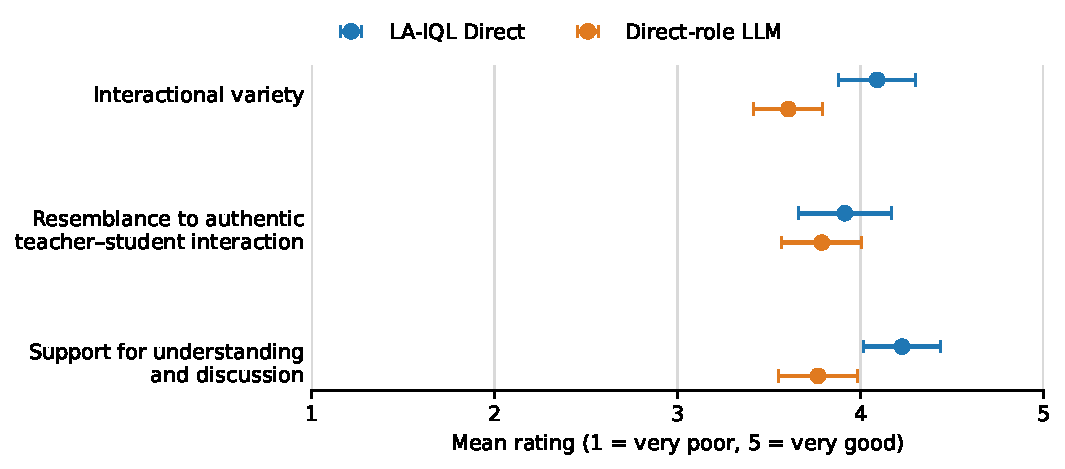
\includegraphics[width=0.86\textwidth]{figure/human_evaluation_two_model.pdf}
  \Description{A two-system dot-and-interval plot for 33 complete responses.
  LA-IQL Direct has higher mean ratings than Direct-role LLM for interactional
  variety and support for understanding and discussion. Their intervals overlap
  substantially for resemblance to authentic teacher-student interaction.}
  \caption{Supplementary excerpt-level human evaluation. Points are means of
  participant-level ratings across six excerpts per system and dimension;
  error bars are 95\% confidence intervals. The figure contains only the main
  LA-IQL Direct system and the Direct-role LLM generation baseline. The first
  and third dimensions differ under Holm-corrected paired tests ($p<.001$),
  whereas perceived resemblance does not ($p=.299$).}
  \label{fig:human-evaluation}
\end{figure*}

\paragraph{Strategy-selection configurations also differ in expressed knowledge structure.}
RQ4 extends the action-level comparisons to the content expressed in generated
dialogue, examining whether strategy-selection configurations are accompanied
by differences in knowledge introduction, connection, and development.
All 250 extracted graphs passed the machine-checkable schema and utterance-ID
evidence constraints. Table~\ref{tab:g4-kg-results} reports the three
prespecified endpoints after first averaging repeated runs within each
system--lesson unit. In addition to the systems used in the main RQ1/RQ2
comparisons, RQ4 includes completed Frozen BC and LoRA BC trajectories and an
LM-likelihood reranking baseline. Full implementation details are reported in
Appendix~\ref{sec:reproducibility}.

\begin{table*}[t]
\centering
\small
\setlength{\tabcolsep}{7pt}
\begin{tabular}{lrrr}
\toprule
System & UER$_{100}$ & Mean relational degree & Late-stage relation growth \\
\midrule
Expert transcript & 14.17 & 1.906 & 0.456 \\
LA-IQL Direct & 23.95 & 2.112 & 0.379 \\
LA-IQL Candidate & 31.14 & 2.116 & 0.379 \\
LA-IQL w/o TD (Direct) & 27.96 & 1.963 & 0.380 \\
Direct-role LLM & 38.65 & 2.159 & 0.334 \\
Constrained teacher prompt & 39.15 & 2.164 & 0.360 \\
Frozen BC & 30.36 & 2.012 & 0.301 \\
LoRA BC & 32.22 & 2.064 & 0.325 \\
Likelihood rerank & 28.32 & 2.202 & 0.335 \\
\bottomrule
\end{tabular}
\caption{Knowledge-graph endpoints for RQ4. UER$_{100}$ is the number of
evidence-grounded unique entities per 100 non-END turns. Generated-system
values first average the three completed runs within each of the 10 held-out
lessons. The expert row contains one transcript per lesson. These endpoints
describe generated knowledge structure, not factuality or instructional
quality.}
\label{tab:g4-kg-results}
\end{table*}

Relative to Candidate, Direct introduces 7.19 fewer unique entities per 100
turns (95\% CI $[-10.43,-4.25]$, Holm-adjusted $p=.0059$), while mean
relational degree ($-0.003$, CI $[-0.098,0.093]$) and late-stage relation
growth ($-0.001$, CI $[-0.065,0.052]$) are nearly unchanged. Relative to the
matched w/o-TD Direct checkpoint, Direct is lower in UER$_{100}$ by 4.00
(CI $[-8.69,-0.05]$, adjusted $p=.2109$), higher in mean relational degree by
0.149 (CI $[0.059,0.240]$, adjusted $p=.0527$), and indistinguishable in
late-stage growth ($-0.001$, CI $[-0.048,0.050]$). These results support the
interpretation that differences between the evaluated strategy-selection
configurations are accompanied by differences in expressed content
organization: Direct introduces fewer distinct entities than Candidate,
with similar observed mean relational degree and late-stage relation growth.
The latter similarities are descriptive and do not establish equivalence.
This extends the comparison beyond action labels, while the system-level
contrast does not isolate strategy selection as the cause of these differences.
UER$_{100}$ has no intrinsic ``higher is better''
direction, so this result should not be interpreted as an educational-quality
ranking.

Appendix~\ref{sec:additional-results} gives the full system-level comparison,
RQ3 table, and judgment status.
 
\section{Discussion}

\subsection{Human Grounding as an Inspectable Design Resource}

Our first contribution is methodological: action mediation renders human
grounding an operational and inspectable design resource for building more
natural interactive agents. The action vocabulary, training demonstrations,
and held-out comparison patterns are all drawn from authentic classroom
interaction. It links policy learning, generation, and evaluation through a
shared human-readable strategy layer. This goes beyond structured prompting for
next-utterance generation: it establishes a stable interface at which designers
can inspect what strategy was selected, how strategies unfold over time, and
how each choice is realized in language. For HCI practitioners seeking to move
beyond agents that merely answer questions toward agents that guide, probe, and
collaborate, such traceability is essential. This is because it distinguishes
between hoping a model has acquired sound interactional habits and verifying
what it has actually learned.

The metric-matched Markov control clarifies what human-pattern alignment can and
cannot establish. Its strong local alignment indicates that transition
similarity can be reproduced without reading the dialogue; the semantic
intervention, by contrast, shows that the learned policy distribution responds
to dialogue content beyond the preserved action history. Human-pattern
similarity is therefore informative only when situated within a broader,
inspectable evaluation rather than treated as a sufficient measure of
context-sensitive interaction. This finding carries a cautionary implication
for the broader enterprise of learning from human demonstrations: matching
surface statistics of human behavior does not guarantee that the agent has
internalized the underlying interactional competence. Human grounding still
does not ensure globally human-like or contextually appropriate behavior, but
the action boundary makes the relevant successes and failures empirically
separable, and therefore addressable.

\subsection{TD-Associated Differences Support a Longer-Horizon Interpretation}

The matched Direct-decoding checkpoint contrast isolates the clearest observed
TD-associated difference. The w/o-TD checkpoint shows no reliably detected
difference in local expert-pattern alignment yet exhibits 53\% more two-step
cycles and 36\% more repeated motifs. This pattern is consistent with the TD
term affecting recurrent sequence organization rather than merely expanding
the action vocabulary or improving one-step imitation, though the single
checkpoint per condition precludes a training-objective-level causal
conclusion. The w/o-TD policy also terminates five of 30 trajectories before the
100-action horizon, whereas the TD policy terminates none, providing further
descriptive evidence of divergent rollout behavior. Because each condition
contains one trained checkpoint, the bootstrap captures held-out lesson and
generation variation but not training-seed uncertainty.

This fixed-checkpoint result supports the analytical value of the
action-mediated formulation for identifying differences in recurrent
interaction organization. It localizes the observed TD-associated difference in temporal organization
(i.e., 53\% more two-step cycles and 36\% more repeated motifs for the evaluated
w/o-TD checkpoint) rather than in local expert-pattern alignment or
action-vocabulary expansion. This distinction bears directly on user
experience: an agent that cycles through a small repertoire of interaction
moves, however locally appropriate, will feel monotonous and predictable in
sustained use. End-to-end text evaluation would obscure this distinction, since
surface-level lexical variation can mask underlying interactional rigidity.
The supplementary excerpt ratings indicate perceived gains in interactional
variety and support for discussion, but they do not establish sustained
coherence, experienced usefulness, or educational benefit. Understanding how
the structural properties translate into extended user experience remains
future work.

\subsection{Action Mediation Makes Control Allocation Observable}

Separating strategy selection from language realization turns control
allocation into an observable design variable. The completed Direct
configuration grants the learned policy access to the full action space and
yields stronger alignment with held-out human action patterns, but also
produces more short cycles and repeated motifs. The Candidate configuration
restricts action support to role-model proposals and exhibits fewer
repetitions, yet its trajectories diverge further from the held-out action
distribution. Because the configurations also differ in rationale temperature,
this constitutes a descriptive system-level contrast. Nevertheless, the
completed configurations illustrate that greater policy control over action
support need not coincide with lower recurrence: strategy support, temporal
organization, and wording must be considered jointly.

This finding has practical implications for how designers configure interactive
agents. The trade-off between alignment and repetition---between faithfully
reproducing human action distributions and avoiding conversational ruts---cannot
be resolved by simply granting the policy more or less control. Rather, it
requires careful consideration of where in the generation pipeline different
constraints should operate. The explicit action boundary provides a concrete
substrate for such structural traceability. It enables system designers to
compare the strategy selected for a state with the utterance ultimately
produced, inspect recurring control patterns, and localize whether a divergence
originates in policy choice or realization. We establish this as a method-level
traceability capability. Nevertheless, for HCI researchers and practitioners
building interactive systems, this form of inspectability is a prerequisite for
responsible iteration and improvement.

\subsection{Implications for Evaluating Interactive Dialogue Agents}

Three implications follow from the present testbed for evaluating interactive
agents that aim to engage in richer, more human-like dialogue. First,
action-pattern metrics should be paired with controls whose inductive biases
match those metrics; otherwise, local statistical reproduction may be mistaken
for context-sensitive competence. An agent that reproduces the local
distribution of human interaction moves may still fail to respond meaningfully
to what has actually been said, a failure that becomes visible only when one
intervenes on the dialogue content itself. Second, evaluation should treat
strategy choice and language realization as separate but coupled objects: an
appropriate action label is of little use when the utterance fails to express
it. Whether the agent intends to guide, challenge, or acknowledge and whether
it actually does so through language is an empirical question, not a given.
Third, long-horizon repetition must be reported alongside diversity and
alignment, because a policy can cover human-supported patterns while repeatedly
cycling among a small subset. For interactive agents deployed in sustained use,
this is precisely the kind of failure that erodes user trust and engagement even
when individual responses appear appropriate.
Recent analysis of authentic student--LLM use likewise shows why evaluation
must reflect how people actually interact with systems rather than only how a
system is intended to be used, and why turn-level and whole-dialogue views are
complementary~\citep{kobler2026students}.

Taken together, these findings suggest an evaluation framework for
strategy-rich interactive agents: expose a readable strategy layer, assess
whether the policy uses interaction context, and evaluate human-pattern
alignment, temporal organization, and language realization as complementary
rather than interchangeable properties. This framework speaks directly to the
HCI community's interest in designing systems that are not merely capable but
genuinely usable and engaging in real human interaction. The action-mediated
approach provides the transparency necessary to shift evaluation from the
question of whether an agent produces fluent responses toward whether it
interacts effectively and whether the basis for that interaction is observable.

\section{Conclusion}

Interactive agents are increasingly embedded in daily life, and dialogue
remains the primary channel through which they serve human needs. Yet the gap
between answering questions well and engaging in genuinely collaborative,
adaptive interaction remains wide. This paper introduced an action-mediated
formulation for learning human-grounded interaction strategies and instantiated
it in LA-IQL. From fixed human interaction trajectories, LA-IQL learns an
explicit policy over readable interaction acts through rationale-conditioned
action prediction and offline inverse Q-learning, while keeping strategy
selection separate from language realization. This formulation makes
interaction decisions, temporal organization, and surface realization
independently inspectable. This is a necessary condition for building agents
that move beyond mechanical responsiveness toward natural, context-sensitive
engagement.

Across held-out long-horizon classroom rollouts, the evaluated TD-regularized
checkpoint produced less recurrent behavior while preserving similar local
human-pattern alignment. In the evaluated inference configurations, varying how
control is allocated between the policy and the role model revealed a trade-off:
direct selection better preserved held-out human patterns, whereas
proposal-constrained re-ranking reduced recurrence. Together, these findings support the claim that action
mediation can reveal consequential differences in interaction organization
that fluent text or local similarity alone can obscure.

The broader significance of this work lies in its treatment of human
interaction as a learnable and inspectable resource. By making strategy
explicit, we enable designers and researchers to pose sharper questions about
what interactive agents have actually learned from human demonstration, how
they organize behavior over time, and where their limitations reside. The
evidence supports an inspectable modeling and evaluation interface for
strategy-rich interactive agents. It is bounded to the evaluated checkpoints,
structural behavior, and short excerpt-level judgments. These boundaries define
the trajectory of future work: extending action-mediated learning to diverse
interactional domains, validating structural properties in sustained user
experience, and ultimately
building interactive agents that do not merely respond to people, but engage
with them.

\label{main-content-end}

\section*{Limitations}

LA-IQL relies on a fixed interaction-act taxonomy derived from one classroom annotation scheme.
The resulting 31-action space may omit pedagogically meaningful behaviors and may not transfer unchanged across subjects, grade levels, languages, cultures, or classroom formats.
Although the framework is designed around domain-specific state and action
spaces and is motivated by a broader interaction-learning problem, this paper
evaluates only its classroom-dialogue instantiation and makes no empirical
transfer claim to other interactive-agent domains, including conversational
assistants, multi-agent systems, or embodied agents.
Because the method learns from offline expert demonstrations, it can reproduce annotation errors and systematic biases in the source corpus and cannot identify effective strategies that are absent from that corpus.
The finite-context policy observation may miss long-range instructional goals even though the role model receives a longer dialogue history.

The completed Direct and Candidate configurations differ in rationale sampling
temperature in addition to their action-selection mechanism. Their comparison
therefore identifies a reproducible system-level trade-off but does not isolate
the causal effect of decoding mode; decoding-specific causal attribution is
outside the claims of this paper.

Generated rationales should not be interpreted as faithful causal explanations of the model's internal computation.
They are supervised textual intermediates and can be plausible while remaining incomplete or inconsistent with the selected action.
The explored proposal-constrained adjustment is limited by candidate coverage: a strong Q-function cannot select an action absent from the proposal set, and it does not distinguish utterances sharing the same action label. Direct decoding avoids this support restriction but delegates realization of its selected action to a separate role model, which may fail to express that action faithfully.
Finally, automatic action-distribution metrics do not establish educational
effectiveness, and this paper makes no claims about learning outcomes or
teacher-training utility.
The supplementary human evaluation uses a small convenience sample, six
same-topic excerpt sets, and a shortened instrument whose A/B/C positions are
not fully balanced. It supports perceived variety and discussion support for
the two generated systems, but does not establish sustained coherence,
engagement, trust, preference, educational usefulness, or learning outcomes.
Authentic transcript ratings are not used for model-comparison inference
because transcription loss and unmatched excerpt length and dialogue state
make them a non-equivalent reference condition.
The RQ4 knowledge-graph endpoints likewise measure structures expressed in
generated text, not changes in student cognition, factual correctness,
instructional quality, or learning outcomes. Machine-checkable schema and
utterance references do not by themselves establish that extracted entities
and relations are semantically correct, and exact edge identities may vary
across repeated automatic extraction.
Moreover, the current alignment endpoints emphasize local action $n$-grams and
transition distributions. A policy such as the first-order Markov control can
score highly by conservatively reusing training-supported transitions without
responding to the semantic content of the current classroom state. Our
50-state intervention provides evidence that the Full policy distribution
changes with utterance semantics, but its deterministic donor and small sample
bound the conclusion to distributional sensitivity rather than contextual
decision quality.

\section*{Ethical Considerations}

Classroom dialogue can contain personal information and involve minors, making privacy, consent, and data governance central to this work.
We use the classroom data in accordance with applicable local regulations. Real identifying information was removed from the transcripts before use, and we will not release the original audio, video, or transcript data.
Adult questionnaire volunteers were informed of the study purpose and data use
before participating voluntarily. Their responses are analyzed in de-identified
form and reported only in aggregate.
Generated dialogue must not be presented as a substitute for qualified teachers or used for high-stakes assessment without human oversight.

An interactive agent built with this framework may reproduce cultural,
linguistic, or pedagogical biases present in the demonstrations and in the
underlying language models.
In particular, a policy trained on a narrow classroom population may incorrectly treat one discourse style as universally expert.
Deployment should therefore include subgroup and cross-context evaluation, educator review, clear disclosure that outputs are machine-generated, and mechanisms for users to contest or override generated recommendations.
LLM-generated rationale annotations also require quality auditing because fluent explanations can conceal labeling errors or unsupported assumptions.

\bibliographystyle{ACM-Reference-Format}
\bibliography{references}

\clearpage
\appendix
\section{Additional Experimental Results}
\label{sec:additional-results}

\subsection{Operational Action Definitions and Examples}
\label{sec:action-definitions}

Table~\ref{tab:action-definitions} expands the compact vocabulary in
Table~\ref{tab:action-space}. The examples are translated and lightly abridged
from de-identified utterances in the source corpus; they illustrate how
the same symbol can be performed by either role. Because annotation is assigned
at the utterance level, an example may also contain conversational material
outside the focal act.

\begin{table*}[t]
\centering
\scriptsize
\setlength{\tabcolsep}{3.5pt}
\begin{tabularx}{\textwidth}{@{}l>{\raggedright\arraybackslash}p{0.29\textwidth}>{\raggedright\arraybackslash}p{0.285\textwidth}>{\raggedright\arraybackslash}X@{}}
\toprule
Symbol & Operational definition & Teacher example & Student example \\
\midrule
Ipk & Prior-known-knowledge question: solicits a standard-answer fact, concept, rule, or method accessible through recall. & ``Which coordinate is zero for a point on the $y$-axis?'' & ``Why are some tree rings wide and others narrow?'' \\
Pk & Prior-known-knowledge response: supplies a recalled fact, concept, rule, or basic method with little further inference. & ``The water tap's motion is rotational.'' & ``Corresponding angles of similar triangles are equal.'' \\
Ipi & Personal-information question: solicits a subjective view, feeling, or interpretation grounded in personal experience. & ``How else could you understand it?'' & ``What did that make you think of?'' \\
Pi & Personal-information response: expresses a subjective view, feeling, or interpretation without requiring objective evidence. & ``I think he went from one mountain to another.'' & ``I want to thank the people who protect animals.'' \\
Ia & Analysis question: requests explanation, analysis, evaluation, or evidence beyond simple recall. & ``Which words in the passage support that reading?'' & ``How can you be sure it has this shape?'' \\
An & Analysis response: provides explanation, analysis, evaluation, or elaborated evidence. & ``The particles are constantly moving.'' & ``Because the tree can withstand life's trials.'' \\
Ic & Coordination question: asks a participant to summarize, compare, connect information, or identify a general pattern. & ``Can you summarize it in one sentence?'' & ``So the zero mark must touch the measured object?'' \\
Co & Coordination response: summarizes, compares, connects information, or states a general pattern. & ``The text describes its appearance, activities, and habitat.'' & ``Thus, the sounds of all four seasons are beautiful.'' \\
Is & Speculation question: asks a participant to infer, transfer, predict, or explore an unknown case from known information. & ``Would the same pattern hold for a cart on a slope?'' & ``What if the triangle were changed to an equilateral one?'' \\
Sp & Speculation response: offers an inference, transfer, prediction, or exploration of an unknown case from known information. & ``Do not light fires in a forest; they can cause a wildfire.'' & ``I also saw a small boat moving quickly.'' \\
Iu & Uptake question: invites further discussion, extension, deeper analysis, or an alternative view of a preceding contribution. & ``Does anyone in your group want to add something?'' & ``What else could be added?'' \\
Up & Uptake response: extends, analyzes, or offers an alternative to a preceding contribution. & ``That is because it is a distinctive feature of Venice.'' & ``The cart moves faster and faster down the slope.'' \\
Ag & Agreement: explicitly accepts, supports, or positively acknowledges a contribution. & ``Good. Are there any other observations?'' & ``Yes---his high status made that possible.'' \\
Qu & Querying: disagrees with, doubts, corrects, or asks for reconsideration of a contribution. & ``That is not precise enough; please try again.'' & ``No angle is defined as right, so the conclusion does not follow.'' \\
Gu & Guide: gives an instruction, direction, prompt, or requested next step. & ``Please verify whether it is this angle.'' & ``Please practise this on your own.'' \\
\bottomrule
\end{tabularx}
\caption{Operational definitions and role-specific examples for the 15
cognitive-act symbols. Crossing these symbols with teacher and student roles,
and adding \texttt{END}, yields the 31-action policy space. Examples are
translated and lightly abridged from authentic source transcripts and are
illustrative rather than normative.}
\label{tab:action-definitions}
\end{table*}
\FloatBarrier

\subsection{Additional Quantitative Results}

\begin{table}[t]
\centering
\small
\setlength{\tabcolsep}{3pt}
\begin{tabular}{lrrrr}
\toprule
Split & Lessons & Turns & Topics & Transitions \\
\midrule
Train      & 35 & 6,352 & 33 & 6,317 \\
Validation & 5  & 1,039 & 5 & 1,034 \\
Test       & 10 & 2,028 & 10 & 2,018 \\
Total      & 50 & 9,419 & 47 & 9,369 \\
\bottomrule
\end{tabular}
\caption{Corpus statistics for the frozen lesson-level split. Topic counts
within rows are distinct counts and need not sum to the corpus total because
one topic name occurs in more than one partition.}
\label{tab:appendix-data-statistics}
\end{table}

\paragraph{Training and inference configurations.}
LA-IQL directly selects the highest-valued action and then obtains one
role-model realization. Candidate re-ranking instead generates six
action--utterance proposals and constrains the policy to actions represented in
that set. This changes the allocation of control between the policy and role
model. It does not retrain the policy. The completed configurations also use
different rationale temperatures (0.0 vs. 0.6), so the comparison below is a
descriptive system-level contrast rather than an isolated decoding ablation.
The w/o-TD Direct condition instead removes only the temporal-difference term
from training and retains the main Direct generation configuration, including
rationale temperature 0.0. Five of its 30 trajectories terminate after the
minimum allowed horizon, compared with none for main Direct.

\begin{table*}[t]
\centering
\small
\setlength{\tabcolsep}{4pt}
\begin{tabular}{lrrrr}
\toprule
Variant & D2 $\uparrow$ & Cycle-2 $\downarrow$ & Motif $\downarrow$ & JSD $\downarrow$ \\
\midrule
LA-IQL w/o TD (Direct) & 0.4118 & 0.2607 & 0.5379 & 0.0835 \\
\textbf{LA-IQL Direct} & 0.4370 & 0.1708 & 0.3957 & \textbf{0.0827} \\
Candidate re-ranking & 0.4478 & \textbf{0.0488} & \textbf{0.1413} & 0.1059 \\
\bottomrule
\end{tabular}
\caption{Checkpoint and inference-time system comparisons on the same held-out
lessons. The w/o-TD row is a fixed-checkpoint training-objective contrast;
Candidate re-ranking reuses the Full checkpoint and is a descriptive system
configuration, not a separately trained baseline. JSD is the paired
lesson-level bigram divergence.}
\label{tab:appendix-ablation-results}
\end{table*}

Figures~\ref{fig:appendix-paired-effects} and
\ref{fig:appendix-learned-system-profile} provide complementary visual
summaries of these comparisons. The first emphasizes paired uncertainty,
whereas the second preserves the reported metric scales and generation-seed-level
variation.

\begin{figure*}[t]
\centering
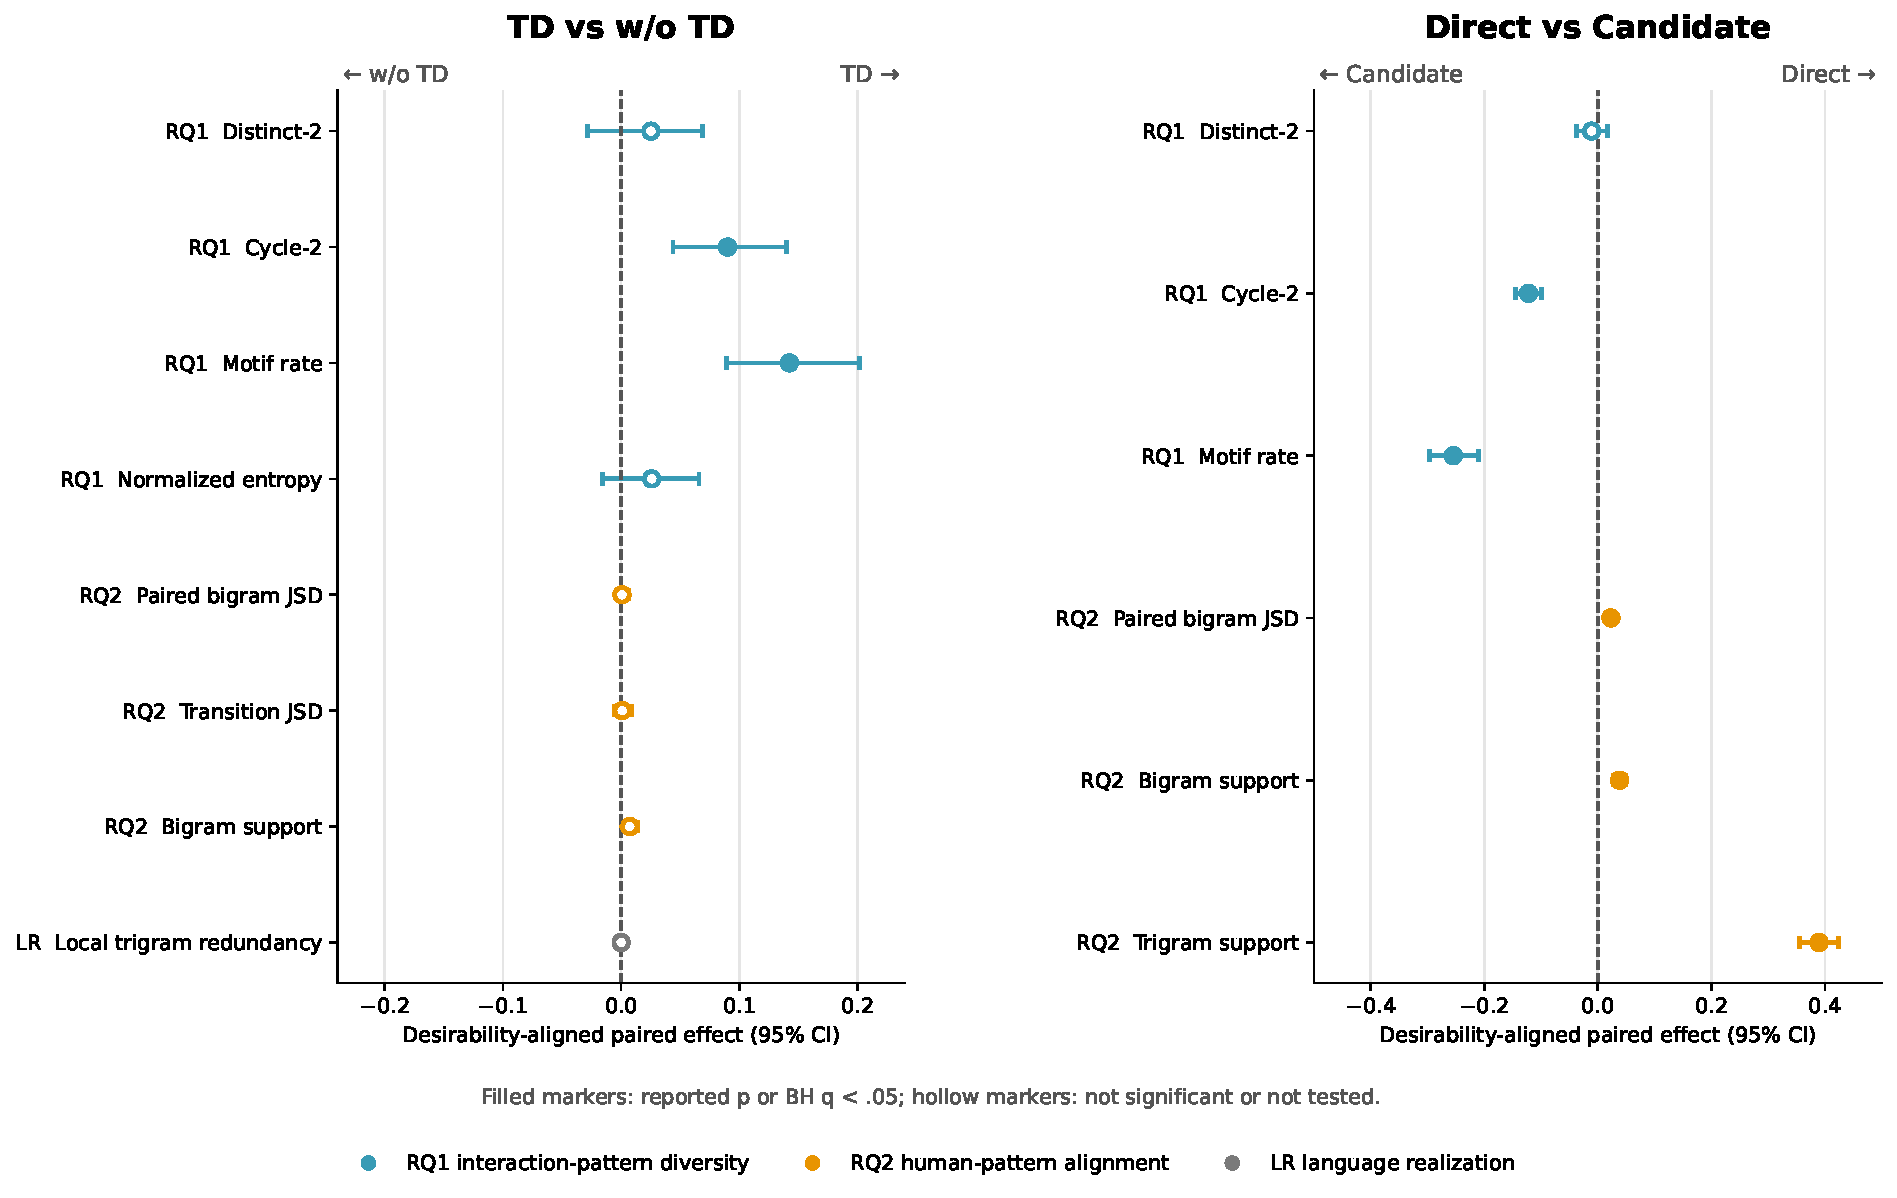
\includegraphics[width=\textwidth]{figure/paired_effects_forest.pdf}
\Description{Two-panel forest plot of desirability-aligned paired effects.
The evaluated TD checkpoint has lower Cycle-2 and motif rate than the checkpoint
without TD. The Direct configuration has higher bigram and trigram support than
the Candidate configuration, while Candidate has lower Cycle-2 and motif rate.
The auxiliary language-realization local-trigram interval and several other
intervals cross zero.}
\caption{Desirability-aligned paired effects for the fixed-checkpoint TD
contrast and Direct--Candidate system contrast. For metrics marked $\downarrow$ in the result
tables, the reported difference and interval are multiplied by $-1$ so that
positive values consistently favor the first named system (TD or Direct).
Horizontal bars are percentile 95\% intervals from 10,000 paired bootstrap
resamples clustered by the 10 held-out lessons. Filled markers denote a
reported $p<.05$ or BH-adjusted $q<.05$; hollow markers denote a
non-significant or untested comparison. The Direct--Candidate panel is a
descriptive system-level comparison because rationale temperature also
differs between configurations. LR marks the auxiliary language-realization
diagnostic rather than an evaluation goal.}
\label{fig:appendix-paired-effects}
\end{figure*}

\begin{figure*}[t]
\centering
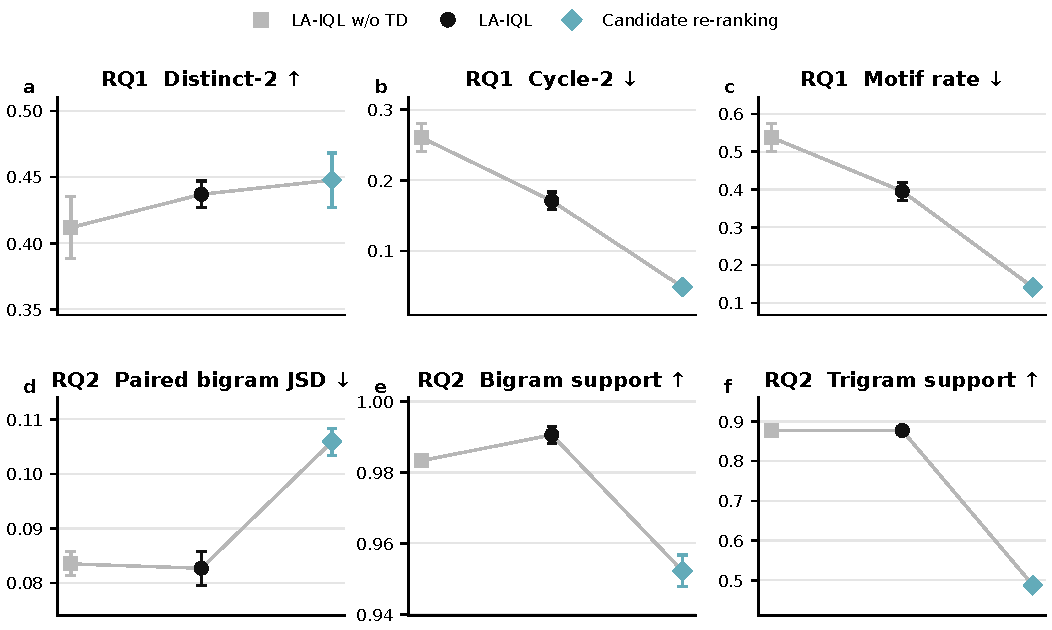
\includegraphics[width=\textwidth]{figure/learned_system_dumbbell.pdf}
\Description{Six-panel point-and-line plot comparing LA-IQL without TD,
LA-IQL, and candidate re-ranking. Candidate re-ranking has the lowest Cycle-2
and motif rates but weaker bigram and trigram support. LA-IQL and its no-TD
ablation have similar paired bigram divergence and support values.}
\caption{Diversity and alignment results for the three LA-IQL configurations (RQ2).
Points show means and error bars show population standard deviations across
generation seeds 42--44 from each fixed checkpoint, with 10 held-out lessons
per seed. Connecting lines are visual
guides rather than temporal trajectories; arrows indicate the desirable
metric direction.}
\label{fig:appendix-learned-system-profile}
\end{figure*}

\paragraph{RQ3 rationale--action simulatability.}
The independent predictor masks action symbols, canonical names,
abbreviations, and deterministic label strings. State and rationale use
separate character 2--5-gram TF--IDF representations and validation-selected
linear classifiers. All three systems use the same frozen evaluator protocol.

\begin{table*}[t]
\centering
\small
\setlength{\tabcolsep}{4pt}
\begin{tabular}{lrrrrr}
\toprule
Method & State F1 & Masked R-only F1 & Combined F1 & $\Delta_{\mathrm{sim}}$ & Accuracy \\
\midrule
LA-IQL w/o TD (Direct) & \textbf{0.0257} & 0.3682 & 0.3629 & 0.3372 & 0.6867 \\
LA-IQL Direct & 0.0159 & \textbf{0.3986} & \textbf{0.4044} & \textbf{0.3885} & \textbf{0.7097} \\
Candidate re-ranking & 0.0123 & 0.1013 & 0.0986 & 0.0863 & 0.2393 \\
\bottomrule
\end{tabular}
\caption{RQ3 rationale--action simulatability. Values are means of the three
generation-seed-level scores. The target is each system's selected action; the result is
an association diagnostic, not a causal-faithfulness measure.}
\label{tab:appendix-g3-results}
\end{table*}

\paragraph{Knowledge-graph evaluation coverage.}
The formal RQ4 extraction contains 250 valid graphs across nine systems, and
all seven prespecified Direct--comparison families have matched lesson-cluster
statistics. The reported evidence is restricted to the three graph endpoints
in Table~\ref{tab:g4-kg-results}; no composite classroom-quality score is
constructed.

\paragraph{Complete diversity and recurrence diagnostics.}
Table~\ref{tab:appendix-full-g1-results} reports the full diversity and recurrence suite for every
completed system. Cov.@20 is the fraction of the 20 expert bigram or trigram
patterns with greatest lesson support (with occurrence count as a tie-breaker)
that appears in a generated run. These diagnostics must be interpreted jointly:
high diversity or low recurrence alone does not imply expert-pattern alignment.

\begin{table*}[!htbp]
\centering
\small
\setlength{\tabcolsep}{4pt}
\resizebox{\textwidth}{!}{\begin{tabular}{lrrrrrrrr}
\toprule
System or control & Runs & Dist.-1 & Dist.-2 & Dist.-3 & Motif $\downarrow$ & Cycle-2 $\downarrow$ & Cov.@20 & $H_{\mathrm{norm}}$ \\
\midrule
\multicolumn{9}{l}{\emph{Generation baselines}} \\
Direct Role LLM & $10\!\times\!3$ & $0.2692 \pm 0.0050$ & $0.4364 \pm 0.0348$ & $0.5913 \pm 0.0427$ & $0.4486 \pm 0.0287$ & $0.0286 \pm 0.0088$ & $0.5500 \pm 0.0408$ & $0.6722 \pm 0.0102$ \\
Constrained Prompt & $10\!\times\!3$ & $0.2866 \pm 0.0029$ & $0.5279 \pm 0.0117$ & $0.7264 \pm 0.0144$ & $0.3403 \pm 0.0204$ & $0.1520 \pm 0.0147$ & $0.5333 \pm 0.0236$ & $0.6818 \pm 0.0015$ \\
\addlinespace
\multicolumn{9}{l}{\emph{Statistical diagnostic controls}} \\
Uniform Random & $10\!\times\!3$ & $0.4149 \pm 0.0198$ & $0.9593 \pm 0.0048$ & $0.9986 \pm 0.0013$ & $0.0048 \pm 0.0012$ & $0.0000 \pm 0.0000$ & $0.3500 \pm 0.0000$ & $0.9287 \pm 0.0066$ \\
Expert Frequency & $10\!\times\!3$ & $0.2154 \pm 0.0145$ & $0.6951 \pm 0.0277$ & $0.9449 \pm 0.0069$ & $0.0795 \pm 0.0098$ & $0.0067 \pm 0.0033$ & $0.9500 \pm 0.0000$ & $0.7144 \pm 0.0111$ \\
First-order Markov & $10\!\times\!3$ & $0.2004 \pm 0.0047$ & $0.5144 \pm 0.0072$ & $0.7815 \pm 0.0026$ & $0.2136 \pm 0.0417$ & $0.0819 \pm 0.0140$ & $1.0000 \pm 0.0000$ & $0.7072 \pm 0.0012$ \\
\addlinespace
\multicolumn{9}{l}{\emph{Learned-policy comparisons}} \\
Frozen BC & $10\!\times\!3$ & $0.0303 \pm 0.0009$ & $0.0694 \pm 0.0062$ & $0.1156 \pm 0.0132$ & $0.9690 \pm 0.0245$ & $0.0072 \pm 0.0069$ & $0.3167 \pm 0.1434$ & $0.2379 \pm 0.0134$ \\
LoRA BC & $10\!\times\!3$ & $0.0250 \pm 0.0085$ & $0.0539 \pm 0.0267$ & $0.0895 \pm 0.0496$ & $0.9697 \pm 0.0173$ & $0.0017 \pm 0.0013$ & $0.3333 \pm 0.2055$ & $0.1267 \pm 0.0940$ \\
\addlinespace
\multicolumn{9}{l}{\emph{LA-IQL checkpoint and inference configurations}} \\
LA-IQL w/o TD (Direct) & $10\!\times\!3$ & $0.1606 \pm 0.0088$ & $0.4118 \pm 0.0236$ & $0.6352 \pm 0.0219$ & $0.5379 \pm 0.0361$ & $0.2607 \pm 0.0193$ & $1.0000 \pm 0.0000$ & $0.6412 \pm 0.0120$ \\
\textbf{LA-IQL} & $10\!\times\!3$ & $0.1663 \pm 0.0034$ & $0.4370 \pm 0.0101$ & $0.6983 \pm 0.0050$ & $0.3957 \pm 0.0240$ & $0.1708 \pm 0.0126$ & $1.0000 \pm 0.0000$ & $0.6670 \pm 0.0084$ \\
LA-IQL + candidate re-ranking & $10\!\times\!3$ & $0.1493 \pm 0.0070$ & $0.4478 \pm 0.0205$ & $0.7221 \pm 0.0238$ & $0.1413 \pm 0.0017$ & $0.0488 \pm 0.0013$ & $0.7000 \pm 0.0408$ & $0.6664 \pm 0.0131$ \\
\bottomrule
\end{tabular}
}
\caption{Complete diversity and recurrence diagnostics for all completed
systems. Values are mean $\pm$ population standard deviation across seeds 42,
43, and 44; each seed contains 10 held-out lessons. BC seeds index independent
training runs and their matching generation runs, whereas LA-IQL configurations
reuse one checkpoint per condition across generation seeds. Diagnostic controls are
included to show that high diversity or low recurrence alone does not establish
expert-pattern alignment; the row groups are not a single fairness-matched
ranking.}
\label{tab:appendix-full-g1-results}
\end{table*}
\FloatBarrier

\section{Implementation and Reproducibility}
\label{sec:reproducibility}

\paragraph{Archived training configuration and provenance boundary.}
We transcribed inference settings from the terminal \texttt{config} object in
the formal trajectory JSON files, data provenance from the frozen split
manifest, and model identity from checkpoint metadata. These artifacts are
authoritative for the reported runs. The recovered run configuration confirms
three two-epoch LoRA stages, the learning rates and loss weights below, physical
batch size 4, one gradient-accumulation step, maximum length 512, gradient
clipping at 1.0, and training seed 42. Full and no-TD share this configuration
except that the Stage~3 TD-loss weight is 1 for Full and 0 for no-TD. The
optimizer details, learning-rate scheduler and warm-up, LoRA rank/alpha/dropout
and target modules, numerical precision, exact sample and optimizer-step counts,
model/tokenizer revision, checkpoint-selection rule, and historical code
revision were not retained in the archived artifacts and are therefore
unavailable for this report. We do not substitute current defaults for those
fields or describe the result as replicated across training seeds.

\begin{table*}[t]
\centering
\small
\setlength{\tabcolsep}{3.5pt}
\begin{tabular}{llrrrrrrr}
\toprule
Stage & Initialization & Epochs & LR & Policy & Cons. & LM-act & TD Full/no-TD & Teacher/self \\
\midrule
1 & Base model & 2 & $10^{-4}$ & 0.25 & 0 & 1.0 & 0/0 & 1.0/0.0 \\
2 & Stage 1 final & 2 & $10^{-4}$ & 1.0 & 0.1 & 0.5 & 0/0 & 0.8/0.2 \\
3 & Stage 2 final & 2 & $5\times10^{-5}$ & 1.0 & 0.1 & 0.5 & 1/0 & 0.6/0.4 \\
\bottomrule
\end{tabular}
\caption{Recovered three-stage configuration for the evaluated Full and no-TD
checkpoints. ``Cons.'' is the cross-head consistency-loss weight and ``LM-act''
is the LM action-class loss weight. The two configurations differ only in the
Stage~3 TD-loss weight among the recovered fields.}
\label{tab:main-training-stages}
\end{table*}

Across Stages 1--3, the recovery-loss weights are 0.5, 0.5, and 0.75; the
action-token weights are 8, 5, and 5; the structure-token weights are 10, 8,
and 8; the rationale-end-token weights are 50, 30, and 30; and the
action-boundary-token weights are 30, 20, and 20. The TD discount is 0.99.
The rationale generator uses maximum 256 new tokens and temperature 0 during
training. Configuration comments that describe micro-batch 1 with accumulation
4 are stale; the actual run parameters are physical batch 4 and accumulation 1.

\begin{table*}[t]
\centering
\small
\setlength{\tabcolsep}{3.5pt}
\begin{tabularx}{\textwidth}{@{}l>{\raggedright\arraybackslash}Xlllll@{}}
\toprule
System & Checkpoint / objective & TD & Selection & Rat. temp. & Role proposals & Randomness \\
\midrule
Full Direct & \texttt{sft\_stage3/final}; four-term objective & on & full-space argmax & 0.0 & one realization & gen. 42--44 \\
Full Candidate & same Full checkpoint & on & six-proposal re-rank & 0.6 & 3/role & gen. 42--44 \\
No-TD Direct & \texttt{sft\_stage3\_woTD/final}; TD removed & off & full-space argmax & 0.0 & one realization & gen. 42--44 \\
Frozen BC & \texttt{sft\_bc\_seed*}; next-action CE & off & full-space argmax & n/a & one realization & train/gen. 42--44 \\
LoRA BC & \texttt{lora\_policy\_seed*}; next-action CE & off & full-space argmax & n/a & one realization & train/gen. 42--44 \\
LM likelihood rerank & \texttt{Qwen/Qwen3.5-0.8B}; no policy training & off & six-proposal LM rerank & n/a & 3/role & gen. 42--44 \\
\bottomrule
\end{tabularx}
\caption{Learned-policy and reranking-system provenance matrix. ``gen.''
denotes generation seeds applied to a fixed checkpoint or inference procedure;
``train/gen.'' denotes independently trained BC checkpoints paired with the
matching generation seed. Both BC systems are included in the formal RQ1/RQ2
action-trajectory comparisons and in the RQ4 knowledge-graph evaluation. The likelihood reranker is an
inference-time baseline and has no trained policy checkpoint.}
\label{tab:system-provenance}
\end{table*}

% Extended provenance record retained in source and omitted from the rendered appendix.
\iffalse
\begin{table}[t]
\centering
\small
\begin{tabularx}{\columnwidth}{@{}>{\raggedright\arraybackslash}p{0.28\columnwidth}>{\raggedright\arraybackslash}X@{}}
\toprule
Artifact & Recorded provenance \\
\midrule
Split & \texttt{g1-formal-v1-deepseek-rationale-rewrite-v1}; seed 20260731; lesson unit; subject--stage strata \\
Source data & source SHA-256 prefix \texttt{5c76ac1d4c2f}; original \texttt{e92eef3da25a}; rewritten \texttt{b18904625ef0}; expert \texttt{7bda9edd0e07} \\
Rewrite & \texttt{rationale-rewrite-v1}; run prefix \texttt{bd7188c66f9a}; 9,168 non-END records in 50 files; 201 END transitions omitted; 8,786/380/2 records accepted on attempts 1/2/3 \\
Full checkpoint & \texttt{Qwen/Qwen3.5-0.8B}; 31 outputs; checkpoint SHA-256 prefix \texttt{a68c26bddc63} \\
No-TD checkpoint & same backbone/output size; checkpoint SHA-256 prefix \texttt{ed0b35180b48} \\
External models & rationale rewrite: \texttt{deepseek-chat}, 0.7, 2026-08-09; role realization: \texttt{deepseek-chat}, 0.8 \\
\bottomrule
\end{tabularx}
\caption{Data, annotation, and checkpoint provenance. Hash prefixes are shown
for readability; the machine-readable manifests retain the full SHA-256 values.
The external API records contain aliases, not immutable provider revisions.}
\label{tab:artifact-provenance}
\end{table}
\fi

\paragraph{Completed BC training metadata.}
The frozen-backbone BC checkpoints use \texttt{Qwen/Qwen3.5-0.8B}, 6,181
training samples, next-action cross-entropy, three epochs, batch size 4,
learning rate $2\times10^{-5}$, and maximum length 512. The LoRA BC checkpoints
use the same backbone, objective, and training set plus 999 validation samples;
they use three epochs, batch size 32, learning rate $10^{-4}$, maximum length
256, rank 8, bfloat16, and one gradient-accumulation step. Each family retains
independent training seeds 42--44 and per-epoch metadata.

\paragraph{Inference configuration and quality gates.}
All reported Full, Candidate, and no-TD formal trajectories use a two-turn,
two-action policy window; a 30-turn, five-action role window; policy maximum
length 512; rationale budget 256 new tokens; horizon 100; role temperature 0.8;
three candidates per role where candidate re-ranking applies; and \texttt{END}
suppression through step 49 with logit margin 3.0. The Full and no-TD
generation gates each contain 50 samples and report 100\% structural validity,
closed rationale/action tags, no degeneration, and no length-limit hits. These
checks establish schema validity, not policy or rationale quality.
Frozen BC and LoRA BC use the same test lessons, horizon, END rule, role-model
temperature, and role-model context; each selected BC action is realized by one
role-model utterance. Their three seed-level runs pair independently trained
checkpoints with matching generation seeds.

\paragraph{Software environment.}
The locked environment requires Python 3.10 or newer and resolves PyTorch
2.11.0+cu128, Transformers 5.14.1, PEFT 0.20.0, scikit-learn 1.7.2, SciPy
1.15.3, OpenAI 2.52.0, and Google GenAI 2.16.0. The dependency lockfile and
CUDA 12.8 wheel index are part of the code artifact.

\section{Context-Sensitivity Intervention}
\label{sec:context-intervention}

The frozen \texttt{context-sensitivity-v1} protocol selects five pre-existing,
evenly spaced held-out states per lesson from the frozen RQ4 candidate pools.
For each state, it constructs a within-lesson cyclic semantic donor while
preserving the number and sequence of speakers and the complete action history.
Rationales are greedily decoded with temperature 0 and a 160-token budget;
\texttt{END} suppression is not applied because this is a state-level test.
Intervals use 10,000 percentile bootstrap resamples clustered by lesson with
seed 20260822.

\begin{table}[t]
\centering
\small
\begin{tabular}{lrrr}
\toprule
Endpoint & Original & Counterfactual & Difference / shift \\
\midrule
Accuracy & 0.4000 & 0.3000 & $-0.1000$ \\
Macro-F1 (31) & 0.1486 & 0.1285 & $-0.0201$ \\
Expert-action probability & 0.2732 & 0.1965 & $-0.0767$ \\
Prediction flip rate & --- & --- & 0.6000 \\
Policy JSD & --- & --- & 0.2957 \\
\bottomrule
\end{tabular}
\caption{Exploratory context intervention for the main Full checkpoint
($N=50$ states, 10 lessons). Lesson-cluster intervals appear in the main text.
The intervention tests distributional sensitivity, not contextual correctness.}
\label{tab:context-intervention}
\end{table}
 
\section{Evaluation Details}
\label{sec:evaluation-details}

Additional diversity and recurrence metrics include Distinct-1/3, repeated local
motifs, and cross-trajectory variance. For RQ3, masking removes action symbols,
canonical names, abbreviations, and deterministic label strings before
prediction. We report leakage rates, per-class scores, confusion matrices, and
majority and shuffled-rationale controls.

The RQ3 evaluation provides association evidence through independent prediction
and within-lesson/role shuffle controls. Its evidential scope is simulatability;
it does not include causal interventions such as removal, paraphrase, or
role-compatible counterfactuals~\citep{deyoung2020eraser}, nor human judgments
of action support or classroom appropriateness. Accordingly, this automatic RQ3 diagnostic does not establish explanation
faithfulness, educational effectiveness, or experienced naturalness. The
supplementary human evaluation separately reports excerpt-level perceptions.

\end{document}
